\documentclass{aa}  
\usepackage{graphicx}
\usepackage{txfonts}
\usepackage{float}
\usepackage[center]{caption}
\usepackage[dashed=false, maxnames=1, uniquelist=false, backend=bibtex,sorting=none,style=authoryear-icomp]{biblatex}
%\renewbibmacro{in:}{}
%\setlength{\bibhang}{0pt}
%\renewcommand*{\bibfont}{\small}
%\renewcommand*{\finentrypunct}{}
\addbibresource{bibliography.bib}
\usepackage{listings}
\usepackage[hyperfootnotes=false]{hyperref}
\pagestyle{plain}
\usepackage{gensymb}

\begin{document} 


   \title{Detection of a transiting Hot Jupiter around WASP-44}
   %\subtitle{}

   \author{Adriana Barbieri
          %\inst{1}
          \and
          Alessandro Bianchetti
          %\inst{1}
          }

    \institute{Dipartimento di Fisica e Astronomia "G.Galilei", Università degli Studi di Padova, Vicolo dell'Osservatorio 3, 35122 Padova, Italy}
             

   \date{February 2022}

% \abstract{}{}{}{}{} 
% 5 {} token are mandatory
 
  \abstract
  % context heading (optional)
  % {} leave it empty if necessary  
   {WASP-44 b is an exoplanet orbiting around its G-type parent star, located in the constellation of Cetus and discovered in 2011 by \cite{Anderson}.}
  % aims heading (mandatory)
   {In this work, we're going to focus mainly on the transit of the exoplanet, in order to retrieve period, radius and time of transit, and we're going to search for any transit time variation signature that may be caused by the presence of a hidden perturbing companion. With this goal, we're going to study and compare two different datasets from TASTE project and TESS mission. We're going to complete the analysis with a radial velocity dataset to yield further insight on the mass and the kinematical properties of the planet. Finally, we make some considerations about the limb darkening effect through different methods (\cite{claret2011},\cite{claret2017}, \cite{claret2018}).}
  % methods heading (mandatory)
   {We first examine stellar atmospheric parameters and derive stellar mass and radius by using \textit{isochrones} (\cite{Morton}). We then analyse some single-night images obtained with Copernico telescope at the ground-based Asiago Astrophysical Observatory and, after proper correction, we use them to extract the light curve of the alleged planet via the TASTE project pipeline. From TESS portal we download another dataset, we select the PDCSAP (Pre-Data Conditioning Simple Aperture Photometry) lightcurve, covering multiple transit events, and we correct for systematics and detrend it. Both TASTE and TESS datasets were analysed with MCMC simulations performed by \textit{PyORBIT}. RV dataset is taken by CORALIE spectrograph on the Euler Telescope in La Silla.}
  % results heading (mandatory)
   {We obtained for our target WASP-44 b a period $P=2.423805\pm0.000021d$, a scaled radius $(R_p/R_{*})=0.1170_{-0.0026}^{+0.0025}$, a mass $M_P=0.88\pm0.07 M_J$ and a density $\rho_p =0.99\pm0.09$ $g/cm^3$.}
  % conclusions heading 
   {We verified %the compatibility of some
   that the main planetary bulk and orbital parameters we retrieved (scaled radius, mass, density, orbital period) are consistent with the ones found in the literature and we also searched for TTV signals in the O-C diagram and in the phase-folded RV curve, finding none.}
   

   \keywords{planet and satellites: detection – TESS – TASTE – CORALIE – star individual: WASP-44 – Techniques: photometric – radial velocities – planets and satellites: individual:    WASP-44 b }

   \maketitle
%
%-------------------------------------------------------------------

\section{Introduction}

Confirmed exoplanets are growing in number year by year, and transit method 
is nowadays a widespread and hugely successful detection method. Most planets 
indeed are discovered 
by tracing the lightcurve and searching for any sign of a weakening in the 
flux.
\begin{figure}[h]
    \centering  
    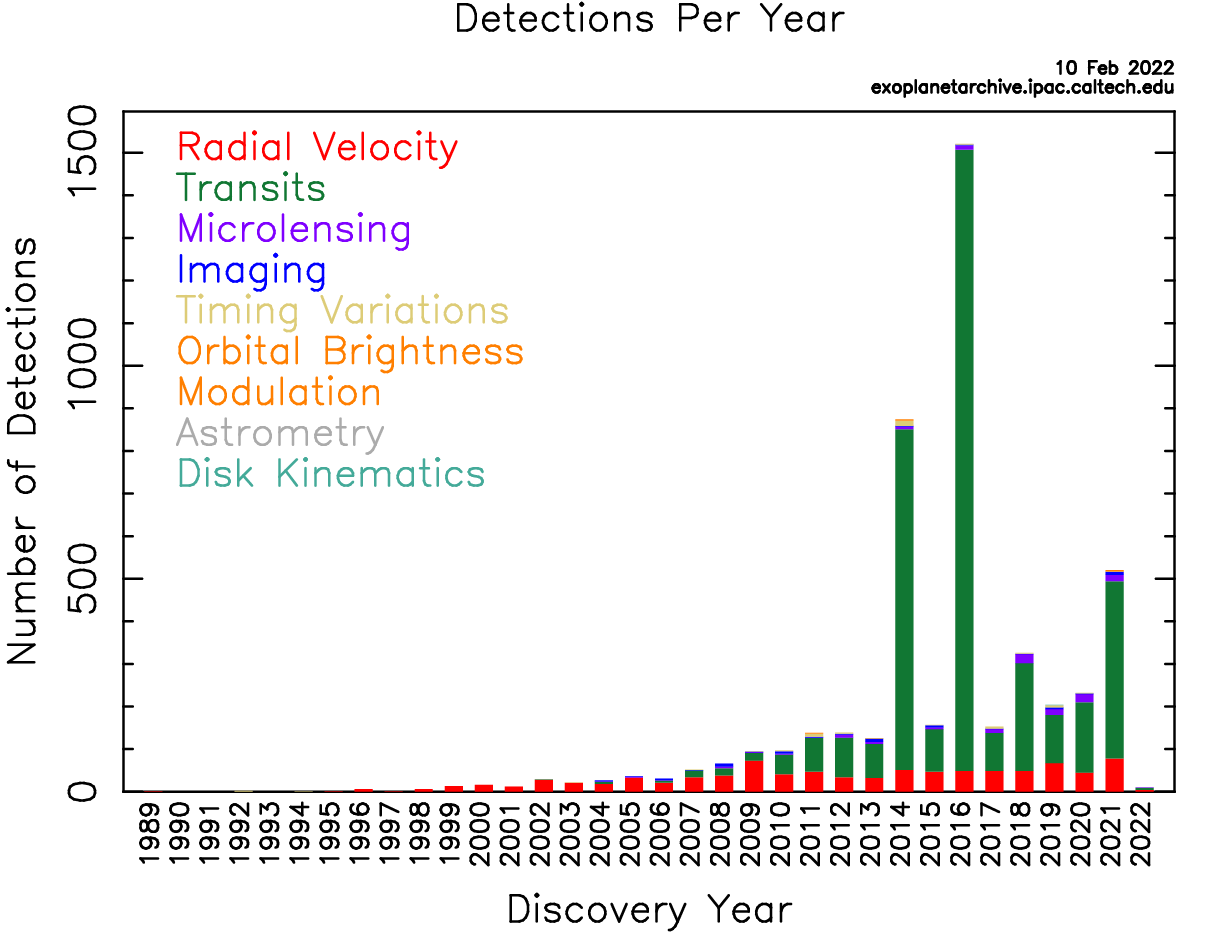
\includegraphics[scale=0.2, angle=0]{pictures/detections.png}
    \caption{Confirmed exoplanets distribution per year of detection via different methods. Credits to \textit{https://exoplanetarchive.ipac.caltech.edu/}}
\end{figure}
In this report we focus on WASP-44 b, a Jupiter-size planet orbiting around 
a G-type star, located in the constellation of Cetus. An estimate of the mass and radius
of the star can be useful for the incoming planetary analysis, but first we need to 
borrow stellar atmospheric parameters from the literature. In a conservative spirit, we avoided any paper result which is not inferred via spectroscopy, and select \cite{Anderson} as our main reference for stellar parameters. This also is the discovery paper of the exoplanet under exam. In this paper, estimates of the atmospheric parameters of WASP-44 are provided via an analysis of the width of the spectral lines.
%\begin{table}[h]
%    \centering
%        \begin{tabular}{cc}
%        \hline
%        Parameter & Value \\
%        \hline
%        $M (M_{\odot})$ & $0.95\pm 0.08$ \\
%        $R (R_{\odot})$ & $0.90\pm0.22$  \\
%        age $(Gyr)$& $0.9^{+1.0}_{-0.6}$ \\
%        $T_{eff}$ & $5400 \pm 150$ \\
%        $\log{g}$ & $4.5\pm0.2$ \\
%        $[Fe/H]$ & $0.06\pm0.10$ \\
%        \hline
%        \end{tabular}
%        \caption{Stellar parameters according \cite{Anderson}}
%    \label{table:00}
%\end{table}
As for the planet WASP-44-b, its main parameters from (\cite{Anderson})
are displayed in \ref{table:0}. 
\begin{table}[h]
    \centering
        \begin{tabular}{cc}
        \hline
        Parameter & Value \\
        \hline
        $M (M_J)$ & $0.889\pm 0.062$ \\
        $P (d)$ & $2.4238039\pm 0.0000087$ \\
        $i (deg)$ & $86.02_{-0.86}^{+1.11}$ \\
      %  $(R/R_{*})^2$ & $0.01588\pm 0.00076$ \\
      %  $(R/R_{*})$ & $ 0.126015872\pm 0.003015493 $\\ from Anderson (propagation)
        $(R/R_{*})$ & $ 0.1260\pm 0.0030 $\\  %rounded
        $b$ & $0.560_{-0.123}^{+0.076}$ \\
        $K (m/s)$ & $138.8\pm 9.0$\\
        \hline
        \end{tabular}
         \caption{Planetary parameters according to \cite{Anderson}}
    \label{table:0}
\end{table}

This work developes as follows: in Section 2 we mention the theoretical frame of the transit method. In Section 3 we present atmospherical and photometric specifics of the target star WASP-44, derive stellar mass and radius and introduce the limb darkening effect, fully addressed in appendix. Section 4 is dedicated to the applied TASTE data pre-reduction pipeline and to aperture synthesis, while in Section 5 we exploit the data already reduced by TESS team, and then perform detrending and transit search. 
% (maybe TESS is pre-reduced and TASTE must be reduced)
Section 6 is focused on a Markov-Chain Montecarlo analysis via a dedicated routine, first for TESS, and then for TASTE with TESS priors. In section 7 we compare the estimated central time of transit from the two datasets, in order to check for transit time variations (TTVs). Section 8 is dedicated to a CORALIE RV dataset analysis, aiming to complete this work with a mass estimate for the planet. In the conclusions, we sum up the main features of the planet.

\section{The transit method }

The transit method is a photometric indirect method of detection of exoplanets, which consists in the observation of a drop in the flux of a star due to the transit of a planet across the stellar disk. 
The subsequent variation of the measured stellar luminosity is proportional to the ratio of the projected areas of the planet and the star, or equivalently, the dimming of the flux is proportional to the ratio of the square of the respective radii; therefore, known the radius of the star from its spectrum, the radius of the planet can be easily obtained from the measured depth of the flux. 

The modelled transit light curve is distinguished by a characteristic trapezoidal shape, whose main geometrical parameters are the impact parameter, the ingress/egress and transit duration, and the transit depth. Also, limb darkening and atmospheric effects may pollute the observational transit curve and cause a deviation from the trapezoidal model.
\begin{figure}[h]
    \centering  
    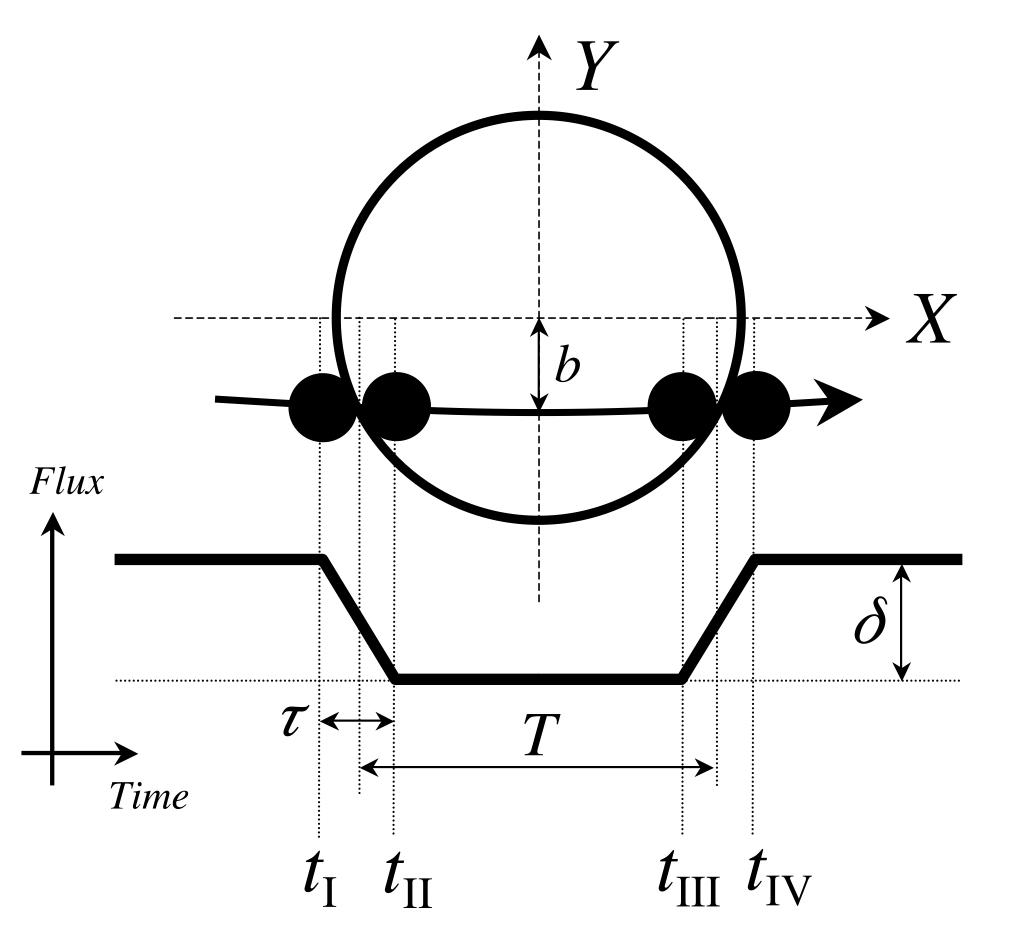
\includegraphics[scale=0.18, angle=0]{pictures/transit.jpeg}
    \caption{Simplified transit light curve. Credits to \textit{Winn [2010]}}
\end{figure}
The geometry of the system places a strong constraint on the inclination of the orbital plane of the planet with respect to the line of sight: the transit can be observed exclusively for almost edge-on orbits, meaning orbital planes that 
are as parallel as possible to the line of sight. This condition yields a low probability of detection, which in turn requires a huge number of target stars to carry on successfull observations. 

Furthermore, at least two transits are required to determine the orbital period of the extrasolar planet candidate, and since the duration of the transit is very short compared to the orbital period, continuous and prolonged observations are required in order to detect it.

It is worth mentioning the selection biases that are intrinsic to this method (and to the current available technology): indeed it yelds the largest detection probability for large planets orbiting very close to small and quiet stars, thus selecting Hot Jupiters around late type stars as ideal targets. Also, one has to look after false positive scenarios, meaning astrophysical phenomena mimicking transit effects, like stellar activity (spots) and stellar companion eclipses.

Transit analysis produces an estimation of planetary radius and orbital inclination: if combined with radial velocities measurements, which provides minimum mass $M_p\sin{i}$, this method yields planetary mass and mean density. The latter, as well as mass and radius, is important to gather information about planet formation and evolution scenarios.




\section{Preliminary steps}

\subsection{Inferring stellar mass and radius}

The $H_{\alpha}$ line was used to determine the effective temperature ($T_{eff}$),
while the $NaI$ D and $MgI$ b lines were used as surface gravity
($\log{g^*}$) diagnostics (\cite{Anderson}). The elemental abundances, including $[Fe/H]$, 
were determined from equivalent width measurements of several clean and 
unblended lines. This led to proper estimation of the atmospheric parameter 
triplet $T_{eff}$, $\log{g^*}$ and $[Fe/H]$. Literature errors include statistical 
uncertainties only. In the same conservative spirit we 
previously showed, we add in quadrature a further term to the errors of 
all three parameters (\cite{Sousa}). 
This leads to the results collected in table \ref{table:a} .
\begin{table}[h]
\centering
    \begin{tabular}{ccc}
    \hline
    $T_{eff}$ (K) & $\log{g^*}$ & $[Fe/H]$ \\
    \hline
    $5400 \pm 162$ & $4.50 \pm 0.22$ & $0.06 \pm 0.11$ \\
    \hline
    \end{tabular}
     \caption{Stellar atmospheric parameters from \cite{Anderson}, with inflated errors.}
\label{table:a}
\end{table}
To run the analysis routine we need also stellar parallax and stellar photometric information. We used Gaia eDR3 parallax $p=2.764 \pm 0.020$ $\mu as$ and retrieved WISE photometric data from IRSA database\footnote{https://irsa.ipac.caltech.edu/Missions/wise.html} in 3 out of the 4 available filters (W1, W2, W3). W4 data were not available for this target. Also, photometry in the J,H and K bands were retrieved from 2MASS catalogue (\cite{2MASS}).
\begin{table}[h]
\centering
    \begin{tabular}{cccc}
    \hline
    WISE & $W_1$ & $W_2$ & $W_3$ \\
    \hline
    & $11.246 \pm 0.022$ & $11.301 \pm 0.021$ & $11.35 \pm 0.19$ \\
    \hline
    \hline
    2MASS & $J$ & $H$ & $K$ \\
    \hline
    & $11.702 \pm 0.023$ & $11.408 \pm 0.025$ & $11.341 \pm 0.026$ \\
    \hline
    \end{tabular}
     \caption{Photometric parameters}
\label{table:star_phot}
\end{table}
We then ran \textit{isochrones} (\cite{Morton}), with Bayesian approach,
with posterior sampling performed by \textit{MultiNest} . The results of the analysis are reported in table \ref{table:b}. Estimated stellar mass is compatible with \cite{Addison}, as well as stellar radius.
%and they are compatible with \cite{Anderson}, who report $M/M_{\odot}=0.95\pm 0.08$ and $R/R_{\odot}=0.90\pm0.22$.
\begin{table}[h!]
\centering
    \begin{tabular}{cc}
    \hline
    Parameter & Value \\
    \hline
     $M (M_{\odot})$ &  $0.95\pm0.05$ \\
     $R (R_{\odot})$ & $0.93 \pm 0.01$  \\
     $\rho (\rho_{\odot})$ & $1.19 \pm 0.09$ \\
     $age (Gyr)$  & $4.8^{+3.5}_{-2.9}$ \\
    \hline
    \end{tabular}
\caption{Stellar physical parameters derived by \textit{isochrones}}
\label{table:b}
\end{table}
Huge errors on the age estimate are pretty common for this analysis, since 
stars with this mass evolve very slowly along the Main Sequence. 

%Mass (Msun)     :     0.952972      0.954230     -0.050431     0.047930
%Radius (Rsun)   :     0.928634      0.928171     -0.011579     0.012578
%Density (ro_sun):     1.192031      1.194963     -0.093708     0.088772
%age (Gyr)       :     4.836685      4.533456     -2.908078     3.512064


%--------------------------------------------------------------------
\subsection{Limb darkening correction}

Limb darkening is an important effect that cannot be neglected when observing a star.
In short, the edges of the luminosity profile 
of a star always look darker than the core: this occurs because there is a physical, constant 
distance $L$ at which the optical depth is equal to unity, further than which 
the observations are not possible since photons are completely absorbed and do not reach the observer. This characteristic size, 
however, can extend deep inside the hot layers of the star if we look straight 
to the center, being $L$ radial, while it only reaches the colder, outer layers 
if we look at the edges of the star, since $L$ and our line of sight (LoS) are not radial 
anymore.
\begin{figure}[h]
    \centering  
    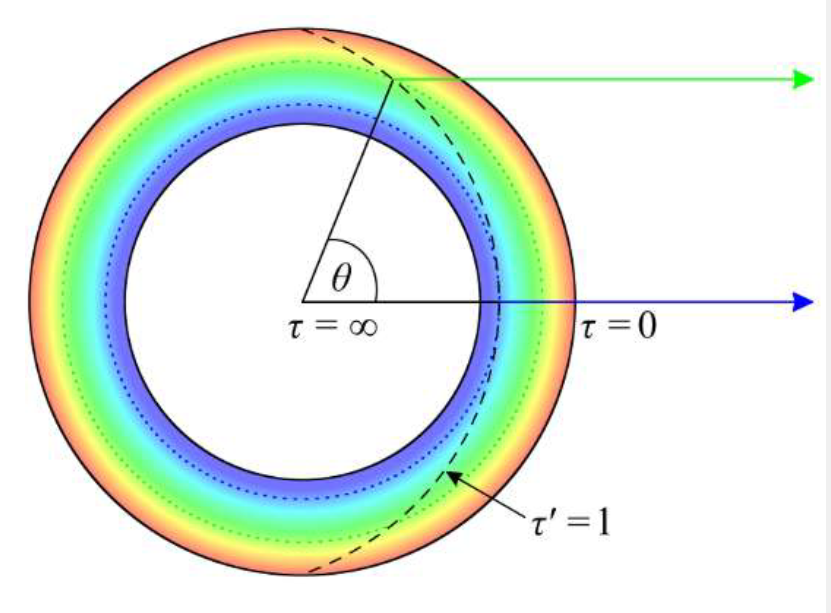
\includegraphics[scale=0.25, angle=0]{pictures/limb_darkening.png}
    \caption{Limb darkening effect scheme. Credits to \textit{https://ediss.sub.uni-hamburg.de}}
\end{figure}
Correcting for this effect may be challenging. Indeed we can measure it 
directly only for the Sun, while we need to model it somehow for any other 
star, thus figuring out a proper law for the intensity decrease $I(\mu)$, 
where $\mu = \sqrt{1-r^2}$. Many choices are plausible at this point: a 
uniform behaviour, a linear, a quadratic, a square-root or a 
logarithmic law are all valid guesses. Parametrizing such laws introduces 
the so-called \textit{LD-coefficients}, which will depend on the stellar 
parameters. Knowing the latter relationship (for instance calibrating it 
based on a large sample of stars) allows to obtain the coefficients directly 
from the atmospheric parameters. 
The alternative way is to fit the light curve leaving the coefficients as free parameters.
Different parametrizations for limb darkening coefficients are possible: throughout the paper, we're going to use Kipping parametrization as a reference (\cite{Kipping}). 

The choice of the functional dependence on
$\mu$ is a delicate one. Multiple modelling approaches can
be followed, based on different papers. This
analysis is addressed in \ref{sect:app_A}, 
where we face three different publications 
by the author Antonio Claret, who provided 
atmospheric parameters tables to calibrate a relationship between limb 
darkening coefficients and atmospheric 
parameters. The oldest paper, \cite{claret2011},
provides a variety of filters from both the Johnson 
system and SDSS, including filter $r^*$, used for TASTE analysis to minimize the atmospheric extinction and limb darkening effects. 
\cite{claret2017} and \cite{claret2018}
are instead referred to the only TESS built-in filter and 
so they're available for comparison with TESS output alone.



\section{TASTE data analysis}

TASTE project\footnote{The Asiago Search for Transit timing variations of Exoplanets} (\cite{Nascimbeni}) provides ground-based observations of our target taken with Copernico 1.82m telescope at the Asiago Astrophysical Observatory, located at Mount Ekar, Asiago (VI), Italy. TASTE goal is to produce a catalog of lightcurves for selected targets using the TTV method. The imaging device is called AFOSC (Asiago Faint Object Spectrograph and Camera), with $9'\times9'$ FoV. Data for WASP-44 were collected between 17:35:02.5' and 21:41:43.7' of 2020 November 20 (UTC), with a 15s exposure time and a $r'$-Sloan filter. The dataset used only contains one transit.

Before actually analysing these data, we need to properly correct them: it is of capital importance to remove instrumental effects in order to largely improve the final result. During observations, targets are defocused on purpose, to avoid saturation and minimizing the effect of pixel inhomogeneity. After proper discussion and conversion into the required format, we will prepare the configuration file for the analysis. 

\subsection{Bias and flat field correction}
CCDs (Charged Coupled Devices) are the favourite detectors for photon counting, 
due to their high quantum efficiency. The images produced are raw
and must be properly \textit{pre-reduced} before being analysed. Pre-reduction goes through different steps:
\begin{itemize}
    \item \textbf{bias} is the additive offset contribution, a zero-exposure instrumental factor. It measures the charges left on the CCD even with the shutter closed and 0 s of exposure time. The presence of these charges is related to the fact that a finite direct current is needed to move the charges from the pixels to the output register, and this introduces a bias in the science frames.  It must be removed in order to isolate the photons of astrophysical origin. The other component of the bias corresponds to the so-called \textit{readout noise}. We will remove the constant DC term and then perform an average of the bias frames to reduce RO noise, that still cannot ever be fully removed;
    \item a \textbf{flat field} is a calibration image obtained by illuminating homogeneously the pupil of the telescope, using twilight sky or appropriate, back-lighted screens. After correcting for bias, flat field correction factor is to be normalised and then applied on each pixel by dividing the science image counts by the estimated pixel efficiency to get to the true counts;
    \item \textbf{differential aperture photometry} allows us to keep track of any noise variation. By normalizing the flux of our target with that of a reference star close enough to it, any first-order systematic trend is cancelled, since any environmental or instrumental variation affects both sources. Therefore all the remaining variations are of astrophysical origin.
\end{itemize}
For pre-reductions steps, we use the \textit{STARSKY} subroutine \textit{HUGGY} (\cite{Nascimbeni}). 

\subsubsection{Bias correction}
30 bias images with $\tau_{exp}=0s$
%and 18390 bias frames
are available, displaying the zero-exposure offset of the pixel board. We run \textit{huggy.bias} to compute the average \textit{master bias} file. We hereby plot a random bias image and the master bias to offer a concrete view of the correction.
\begin{figure}[h]
    \centering  
    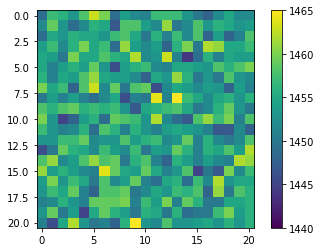
\includegraphics[scale=0.35, angle=0]{pictures/bias.png}
    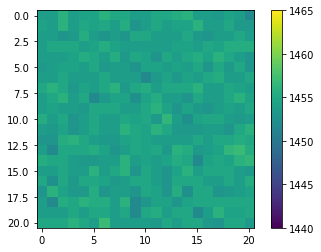
\includegraphics[scale=0.35, angle=0]{pictures/master_bias.png}
    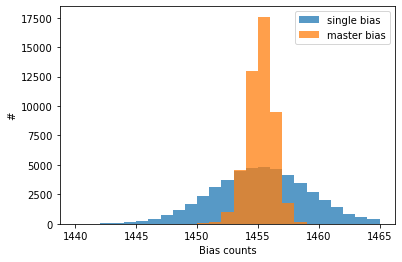
\includegraphics[scale=0.45, angle=0]{pictures/bias_comp.png}
    \caption{Comparison between TASTE random bias frame and master bias}
\end{figure}
Note that the master bias frame distribution is peaked and much closer to a unique constant value, as all pixels behaved in the same way, like in an ideal situation. We can see this even numerically, by looking at the dispersions of the above distributions: $\sigma_{rb} = 3.82$ and 
$\sigma_{mb} = 0.89$.

\subsubsection{Flat field correction}
30 flat field frames with $\tau_{exp}=2s$ are used. We run \textit{huggy-flat.e} inputting a 90\% normalization fraction, meaning the fraction of pixels we want to account for, ruling out the sides which are often polluted by overscan columns. These are visible in the form of dark stripes on the sides of any flat field taken. Then we have to input the overscan values, set to 0 as we do. Subsequently, we need to provide the master bias file, which will be subtracted from the data. Finally, we input all available flat fields. This will produce an output file showing the average response of pixels to an external light source. A normalised version of the file yields the efficiency of each pixel.
\begin{figure}[h]
    \centering  
    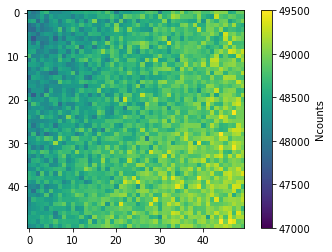
\includegraphics[scale=0.35, angle=0]{pictures/flat.png}
    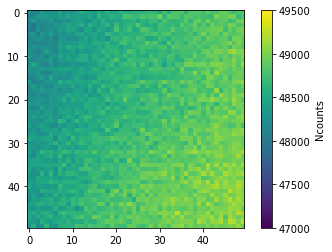
\includegraphics[scale=0.35, angle=0]{pictures/master_flat.png}
    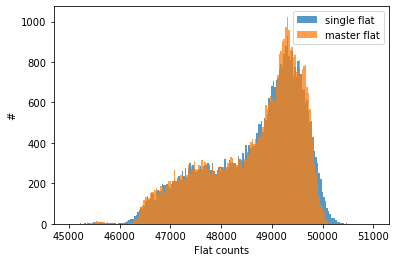
\includegraphics[scale=0.45, angle=0]{pictures/flat_comp.png}
    \caption{Comparison between TASTE random flat field and master flat}
\end{figure}

\subsection{Final correction}
%MISSING NUMBER OF SCIENCE IMAGES
The final step is to apply the correction files obtained in the 
previous sections to science images. The final correction code requires the master bias and the normalised master flat, and of course all the 883 target images ($\tau_{exp}=15s$). First we subtract the master bias (instrumental noise) and then we divide the pixels by the normalised master flat, thus retrieving an estimate of the actual photon counts. All this is done by running \textit{huggy.correct.e}.
The corrected images are now ready for aperture synthesis.


\subsection{Extracting the light curve}
We are approaching the very heart of TASTE analysis, preparing for 
aperture synthesis. We now need to display the science images, make
sure to identify the correct target and select a proper background 
analysis around it. To do that, we used \textit{ds9} to define an inner and outer radius: the former marks a circular region hosting the target, the latter defines a surrounding annulus, that is going to be the sky background reference.

The same procedure must be repeated (with the same inner and outer radii) on a properly selected reference star, close to and roughly as bright as the target. 

The Equatorial J2000 coordinates from IRSA Archive \footnote{https://irsa.ipac.caltech.edu/} for our host star WASP-44 and the chosen reference star are, respectively, RA = 00h 15m 36.77s, DEC = -11d 56m 17.3s and RA = 00h 15m 33.14s, DEC = -11d 54m 27.6s.

The r-Sloan photometric magnitudes for target and reference star are respectively $m = 13.021\pm0.005$ $mag$ and $m = 13.058 \pm 0.005$ $mag$, taken from CDS Portal \footnote{https://cds.u-strasbg.fr/}, thus fulfilling the need of two similar stars for differential photometry.

We report instead in table \ref{table:c} the coordinates from ds9 of the target and of the chosen reference star expressed in pixel units.
\begin{table}[h!]
\centering
    \begin{tabular}{ccc}
    \hline
     & $x_c$ & $y_c$ \\
    \hline
    Target    &  170  &  37    \\
    Reference & 288 & 57  \\
    \hline
    \end{tabular}
\caption{Target and reference star coordinates}
\label{table:c}
\end{table}
%    \medskip
\begin{center}
    $R_{in} = 11$, $R_{out} = 20$
\end{center}
\textit{huggy-psf.e} processes the coordinates of the center of the target, the inner and outer radii, and the corrected science images, yielding information about the Point Spread Function, meaning the flux distribution as a function of the distance from the source core. The ouput displays the radii at which we find 68, 90, 95 and 99\% of the total flux. We're not going to use the 68\% aperture option in this analysis. The remaining three apertures in pixel units are $a_0=4.71$, $a_1=5.97$ and $a_2=8.76$ respectively. 
%    re-estimated x (pix):  169.85
%    re-estimated y (pix):   37.69
Photometry analysis is carried out by another subroutine, \textit{sentinel.e}, which requires the coordinates of the target and of the reference stars, followed by the radii of two selected apertures from the previous output. Also, we need again inner and outer radii of the selected region for the analysis, as well as the fully corrected science images. A centroiding method is also required (we selected the Gaussian option). For a star fainter than average like ours ($J\approx 11$) the recommended choices for the apertures are 90 and 95\%, in order to make sure not to run into saturation. However, all three possibilities were tested. 

\medskip

\textit{sentinel} output is the starting point for TASTE analysis. This file contains main photometric information about target, reference star and sky flux throughout the observation session. (Fig.\ref{fig:sky-ref}). Time was converted from JD (UTC) to BJD (UTC) (\ref{sect:app_B}).
\begin{figure}[h]
    \centering  
    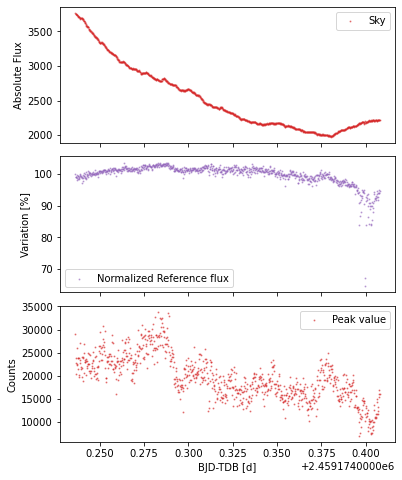
\includegraphics[scale=0.5, angle=0]{pictures/sky-ref.png}
    \caption{Upper panel: sky background flux, every point is the median of the anulus bound by $R_{in}$ and $R_{out}$. Middle panel: reference star flux, normalised to the first measurement. Bottom panel: peak points of the flux inside the defined aperture.}
    \label{fig:sky-ref}
\end{figure}
The sky flux has been constantly decreasing in time, so we expect less and less disturbance as the observation proceeds. The reference star, on the other hand, seems to be pretty stable in terms of flux. We also want to make sure that reference star are correctly comoving with the target: to do that, 
we plot the variation in position at every time step and make sure we have similar motion (Fig.\ref{fig:target-ref_position}). Plotting FWHM reveals an increasing trend, at odds with the sky pattern.
\begin{figure}[h]
    \centering  
    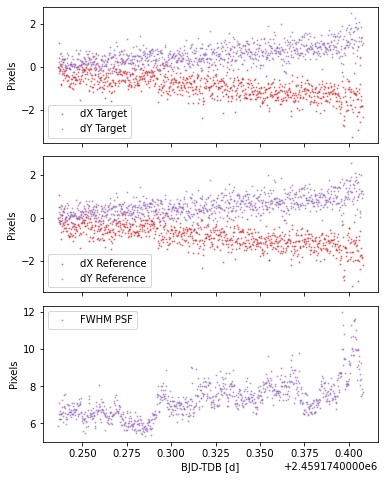
\includegraphics[scale=0.5, angle=0]{pictures/target-ref_position.png}
    \caption{Upper and middle panel: target and reference star show the same coordinate variation in the CCD. Bottom panel: full width half maximum of the peak flux.}
    \label{fig:target-ref_position}
\end{figure}
Next, we compare the flux plot of all three different aperture we have chosen (Fig.\ref{fig:apertures}).
\begin{figure}[h]
    \centering  
    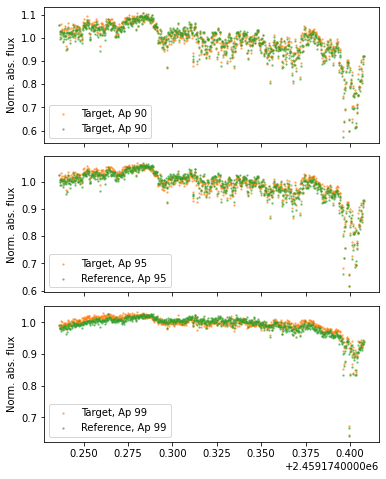
\includegraphics[scale=0.5, angle=0]{pictures/apertures.png}
    \caption{From top to bottom: TASTE 90, 95 and 99\% apertures, showing both the target and reference star. Dispersion is reduced as the aperture grows.}
    \label{fig:apertures}
\end{figure}
The third case (99\%) seems to be slightly less noisy: that's our first clue that this aperture might be the best suited choice for the aperture analysis.
As a further goodness check, one may take a look at the peak value trend of the target source and compare it to the saturation level
(Fig.\ref{fig:saturation-quality}). We also plot the reference star flux to see whether they are above the quality threshold (\ref{fig:saturation-quality}).
\begin{figure}[h]
    \centering  
    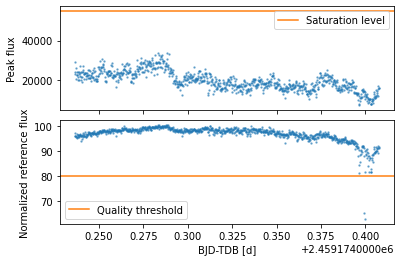
\includegraphics[scale=0.5, angle=0]{pictures/saturation-quality.png}
    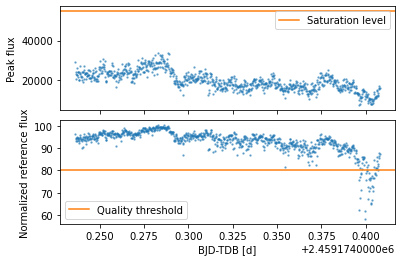
\includegraphics[scale=0.5, angle=0]{pictures/saturation-quality2.png}
    \caption{TASTE apertures. Upper panel: widest aperture, bottom panel: narrowest aperture. In both cases the peak value is well below the saturation limit, and we also see that the reference data are above the required threshold. A few points at late times are below the quality factor in the 90-95\% case, thus supporting the choice of the widest aperture at 99\%.}
    \label{fig:saturation-quality}
\end{figure}
We can can finally visualize the transit in all three cases (Fig.\ref{fig:transits}). To do that, we plot the ratio between target and reference star: \textit{differential photometry} helps us get rid of systematic errors affecting both sources. Once again, we see that 99\% aperture seems to have less dispersion than the other cases.
\begin{figure}[h]
    \centering
    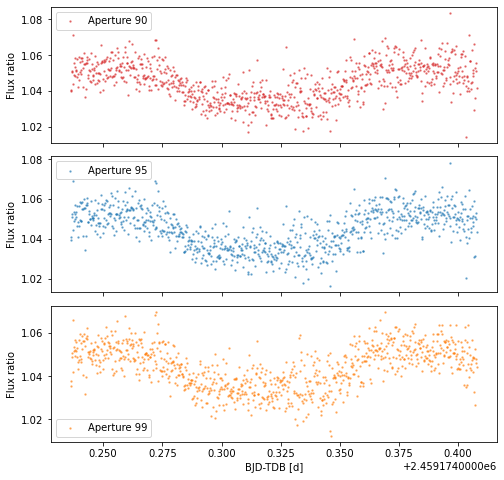
\includegraphics[scale=0.4, angle=0]{pictures/transits.png}
    \caption{TASTE transit image for growing aperture, top to bottom. Note that the above case (90\%) shows the most outliers.}
    \label{fig:transits}
\end{figure}
In-transit datapoints are ruled out to perform a polynomial fit, that will be our reference trend for the stellar flux. The scatter of the fit can help us disentagle between the three apertures, 
\begin{figure}[h]
    \centering  
    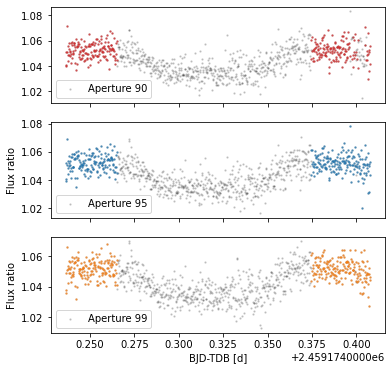
\includegraphics[scale=0.5, angle=0]{pictures/fit_setting.png}
    \caption{Time boundaries for the TASTE transit are roughly ballparked to prepare a proper, flat dataset to fit with a second degree polynomial.}
    \label{fig:fit_setting}
\end{figure}
To rule out transit points, we roughly select an ingress and egress time (Fig.\ref{fig:fit_setting}). A quadratic law ($p_0 x^2 + p_1 x +p_2$) was chosen to set things up in the most general case. A least square fitting via numpy function \textit{np.polyfit} yields the values collected in table \ref{table:d} .
%Fig.\ref{fig:fit} .
\begin{figure}[h]
    \centering  
    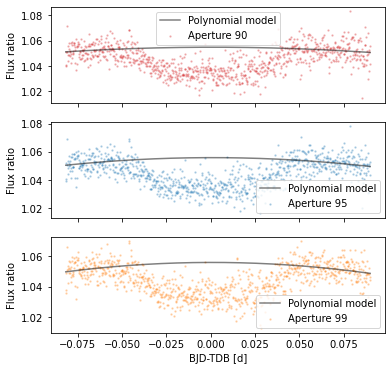
\includegraphics[scale=0.45, angle=0]{pictures/fit2.png}
    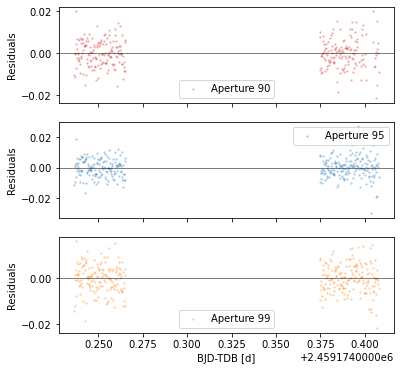
\includegraphics[scale=0.45, angle=0]{pictures/residuals2.png}
    \caption{Polynomial fit on TASTE flux and residuals for the three aperture cases. Before doing the fit, data were shifted so that the central time was placed approximately to zero.}
    \label{fig:fit2}
\end{figure}

\begin{table}[h!]
\centering
    \begin{tabular}{cccc}
    \hline
    \# ap & $p_0$ & $p_1$ & $p_2$ \\
    \hline
    90 & $-0.53$ & $0.0014$  & $1.05$\\
    95 & $-0.80$ & $0.0012$  & $1.06$\\
    99 & $-0.91$ & $0.0014$  & $1.06$\\
    \hline
    \end{tabular}
\caption{TASTE polynomial fit parameters}
\label{table:d}
\end{table}
We immediately notice that the linear coefficient $p_1$ is well compatible with zero. The offset term represents the flux continuum.
%After the fit, we also considered discarding outliers: however, a quick analyisis reveal that all point are well within $5\sigma$, with $\sigma$ being the standard deviation, reported in table \ref{table: f}. Actually, except for the 90\% aperture, even a more strict $3\sigma$ criterion would not rule out any data point.
We display in table \ref{table: f} the standard deviation of the points of the continuous with respect to the linear fit.
\begin{table}[h!]
   \centering
    \begin{tabular}{cc}
    \hline
    $\sigma_{90}$ & $0.0063$ \\
    $\sigma_{95}$ & $0.0061$ \\
    $\sigma_{99}$ & $0.0059$ \\
    \hline
    \end{tabular}
    \caption{Standard deviation of TASTE polynomial fit for three the selected photometric apertures}
\label{table: f}
\end{table}
These quantify scattering and indicate that the 99\% aperture is indeed the best photometric choice, having the smallest standard deviation.



\section{TESS data analysis}
%Conversion from fit parameters to physical parameters

TESS (Transiting Exoplanet Survey Satellite) space mission was launched on April 18, 2018, aboard SpaceX Falcon 9. Its main goal is to search for transiting planets orbiting relatively bright stars (V<11). During its 2-years nominal mission, TESS observed 26 different sectors, each $24\degree \times 96\degree$ wide and observed for a time span of 27 days. Full sky images are provided with a cadence of 30 minutes, while target pixel files (TPF) are obtained pointing at pre-selected targets, observed with a cadence of 2 minutes.
WASP-44 was observed by TESS in $120 s$-cadence mode during observations of sector 3, between 2018 September 20 and October 17. The photometric observations for WASP-44 were reduced by the Science Processing Operations Center (SPOC) pipeline (\cite{Jenkins}):
%https://it.overleaf.com/project/61f1c6cb353cf6130193b1d4s})
all results are available on the MAST platform (Mikulski Archive for Space Telescopes)\footnote{https://mast.stsci.edu/portal/Mashup/ Clients/Mast/Portal.html}.
From ExoFOP-TESS\footnote{Exoplanet Follow-up Observing Program for TESS website, to be found at https://exofop.ipac.caltech.edu/tess/} we retrieved the TIC (TESS Input Catalog) identification number for our target star (12862099).
We were then able to access MAST and download the TESS 2-min cadence TPF, which is a 11x11 pixels cutout centered in the target, produced via the \textit{Lightkurve}\footnote{https://github.com/lightkurve/lightkurve} package for Kepler and TESS.
We performed a preliminary contamination check with \textit{tpfplotter}\footnote{https://github.com/jlillo/tpfplotter.git}, aiming to establish whether our default photometric aperture includes any contaminant star that may cause a dilution of the transit. By running \textit{tpfplotter} we obtained Fig.\ref{fig:tpfplot}, which shows how only one star is present within the aperture, but since it is over 4 magnitudes fainter than the target in the G band, it does not constitutes a contaminant and can therefore be ignored.
\begin{figure}[h]
    \centering
    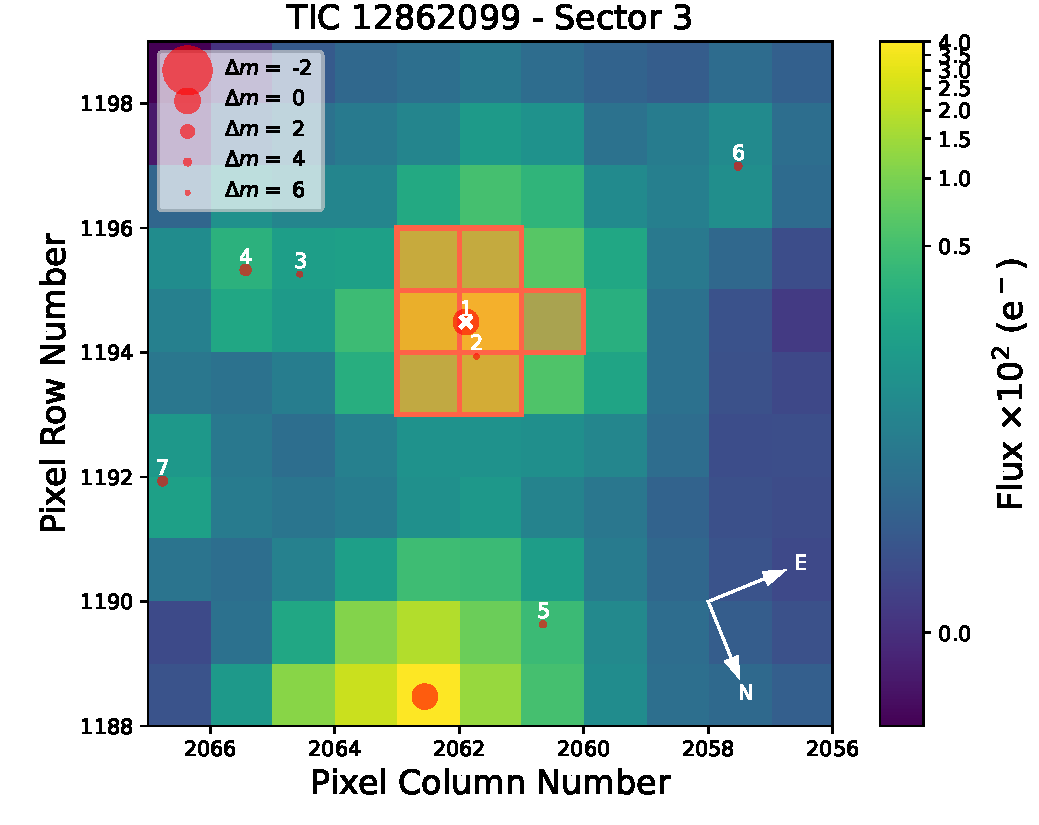
\includegraphics[scale=0.4, angle=0]{pictures/TPF.pdf}
    \caption{TPF plot. The featuring contaminant is faint enough to be neglected.}
    \label{fig:tpfplot}
\end{figure}
We use the mask provided by TESS science team (Fig.\ref{fig:masked_tpf}). 
\begin{figure}[h]
    \centering
    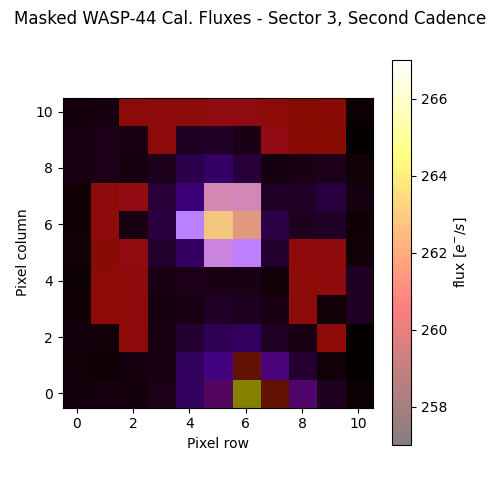
\includegraphics[scale=0.45, angle=0]{pictures/masked_tpf.png}
    \caption{Masked TPF}
    \label{fig:masked_tpf}
\end{figure}

\subsection{Light curve extraction via aperture photometry}
SPOC pipeline yields two lightcurves: SAP (Simple Aperture Photometry), which is corrected for background only, and PDCSAP (Pre-search Data Conditioning Simple Aperture Photometry) which is corrected for any systematics.

We proceeded to perform aperture and time series photometry on the TPF in order to select only the pixels belonging to the optimal aperture; from the obtained calibrated pixels, we derived the transit and the background flux light curves.

Afterwards, we removed from the time series dataset of the optimal aperture all the TESS cadences flagged as anomalous (flag>0) or encoded as NaN. The list of bits that were checked for anomalies is reported in table \ref{table:flag} and further information on flagged data can be found in TESS Science Data Product Description Document\footnote{https://heasarc.gsfc.nasa.gov/docs/tess/documentation.html}.
\begin{table}[h!]
   \centering
   \resizebox{\columnwidth}{!}{
    \begin{tabular}{ccc}
    \hline
    Bit & Value & Description \\
    \hline
    1 & 1 & Attitude Tweak\\
    2 & 2 & Safe Mode\\
    3 & 4 & Spacecraft is in Coarse Point\\
    4 & 8 & Spacecraft is in Earth Point\\
    5 & 16 & Argabrightening event\\
    6 & 32 & Reaction Wheel desaturation Event\\
    8 & 128 & Manual Exclude. The cadence was excluded because of an anomaly\\
    10 & 512 & Impulsive outlier removed before cotrending\\
    12 & 2048 & Straylight from Earth or Moon in camera FOV (predicted)\\
    13 & 4096 & Scattered Light Exclude (spoc-4.0.5 and later)\\
    \hline
    \end{tabular}
    }
    \caption{Data quality flags}
\label{table:flag}
\end{table}
The result of this quality selection can be seen in Fig.\ref{fig:tess}.
\begin{figure}[h]
    \centering
    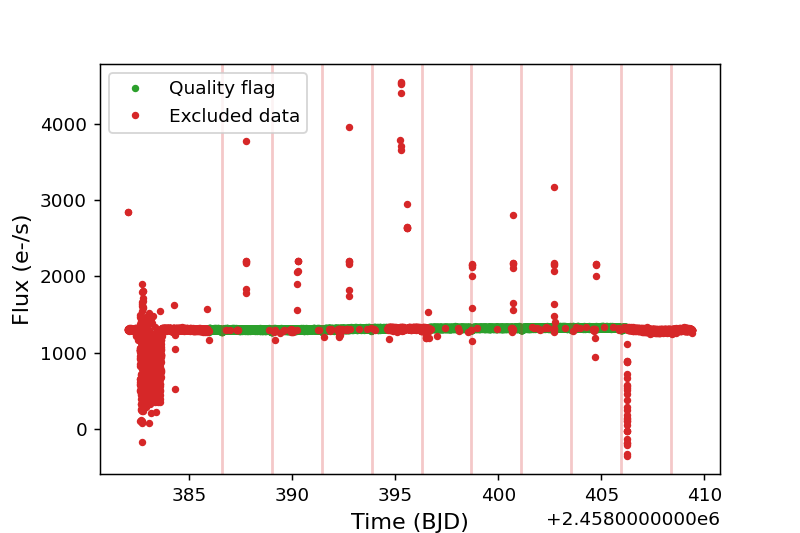
\includegraphics[scale=0.3, angle=0]{pictures/tess.png}
    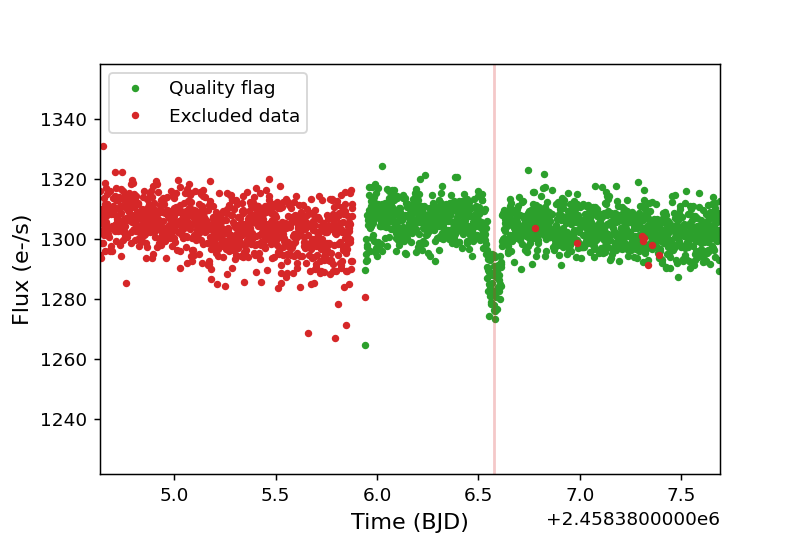
\includegraphics[scale=0.3, angle=0]{pictures/zoom.png}	
    \caption{Flux derived from the calibrated pixels (up) and detail of the first cadence (bottom).}
    \label{fig:tess}
\end{figure}
Subsequently we repeated the quality selection analysis on the lightcurve files (provided by the TESS team and obtained from the MAST portal as previously addressed), and plotted both the optimal 
aperture, the SAP and the PDCSAP fluxes thus obtained as a function of time (Fig.\ref{fig:tess_lc}). 
The observed overlapping between the optimal aperture and the SAP lightcurve is evidence for the goodness of the lightcurve extraction we performed. For our photometric analysis, however, we will make use of the PDCSAP light curve, being it usually cleaner than the SAP flux and also corrected for systematic trends.
\begin{figure}[h]
    \centering
    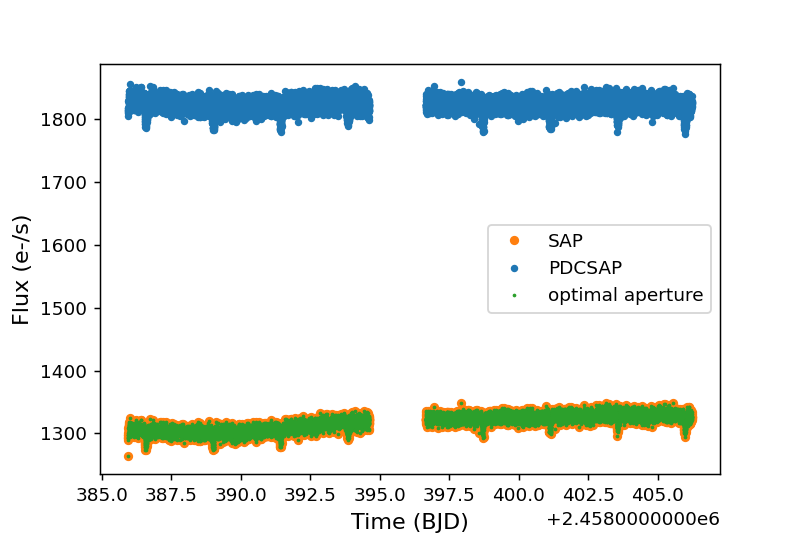
\includegraphics[scale=0.3, angle=0]{pictures/lightcurve.png}
    \caption{Optimal aperture, SAP and PDCSAP lightcurves.}
    \label{fig:tess_lc}
\end{figure}


\subsection{Detrending methods}

It is of capital importance to flatten and de-trend the PDCSAP lightcurve, meaning to correct for stellar activity, 
flares, gaps in the data and interrupted transits by removal of the curve modulation due to the stellar and instrumental systematics.
Via the \textit{WOTAN} package \footnote{https://github.com/hippke/wotan} (\cite{Hippke1}) we applied to the 
PDCSAP light curve a biweight filter with a time window of 1 d and a hspline filter with a time window of 2 d 
(\ref{fig:filters}); afterwards we normalized and folded the lightcurves, with the aim of studying the transits in phase (\ref{fig:Transits}).
\begin{figure}[h]
   % \centering
    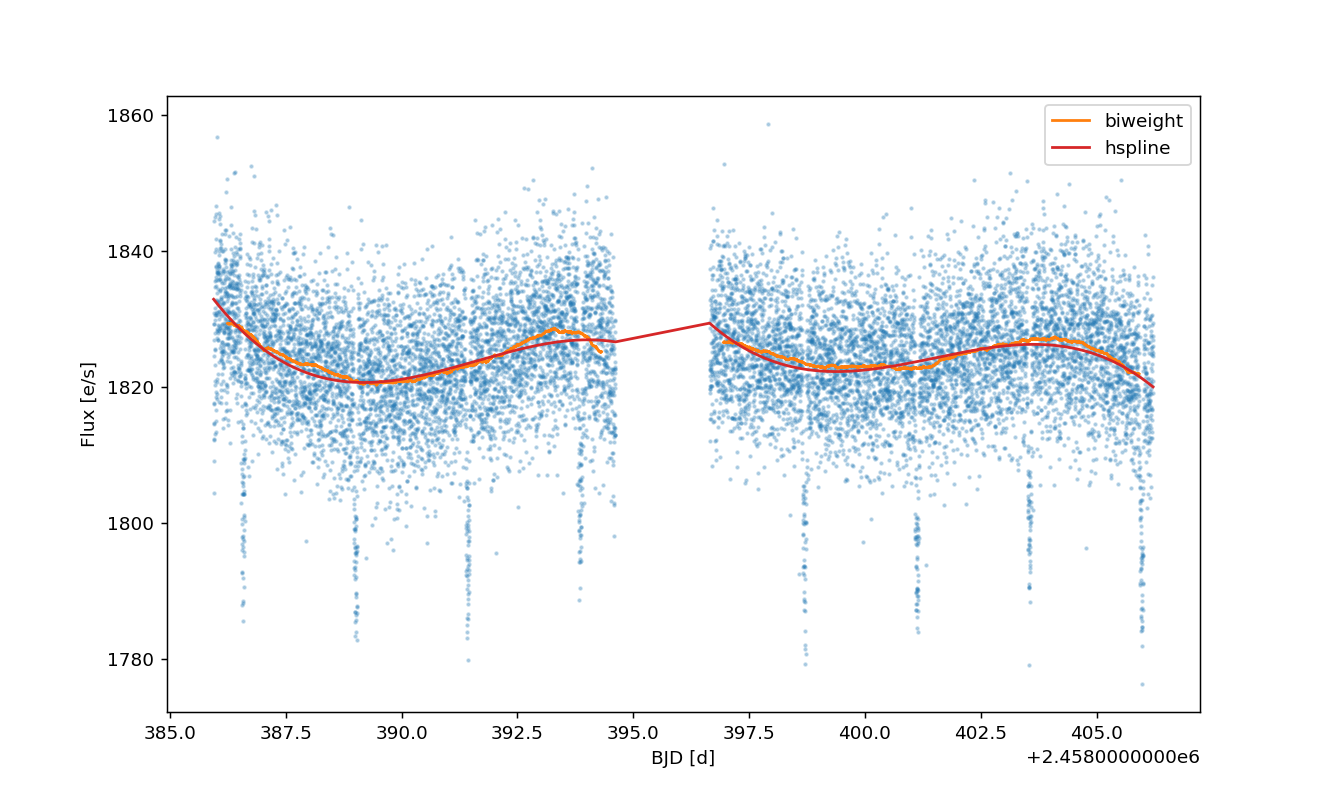
\includegraphics[scale=0.2, angle=0]{pictures/filters.png}
    \caption{Hspline and biweight filters.}%Outliers exclusion and time windowing
   \label{fig:filters}
\end{figure}
\begin{figure}[h]
  %  \centering
    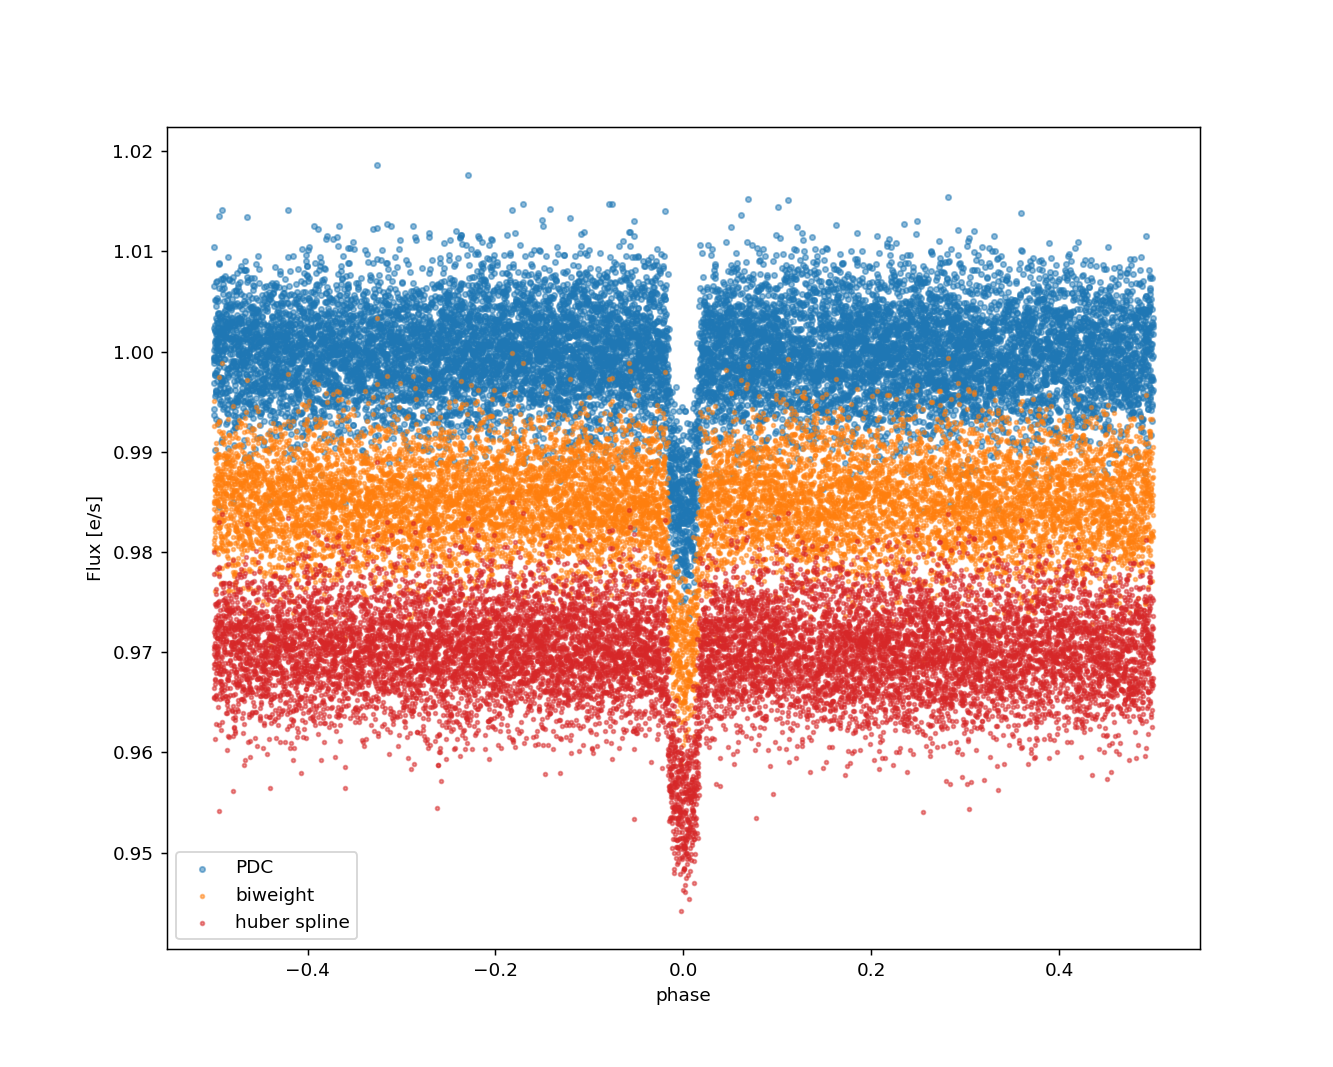
\includegraphics[scale=0.18, angle=0]{pictures/phase.png}
    \caption{Flattened and folded data. With respect to \ref{fig:filters} the difference in flux can be now appreciated}
   \label{fig:Transits}
\end{figure}
We obtained for the PDCSAP, biweight and hspline fluxes' standard deviations the values of %0.00440736, 0.00406469 and 0.00407942 
0.00441, 0.00406 and 0.00408 respectively.
Therefore, having the smallest $\sigma$, we considered the flattened biweight lightcurve as the most accurate one.

\subsection{Identification of periodic signals}

We proceeded to perform an iterative  transit search on the detrended light curve in order to independently confirm the detection of the periodic signals in the TESS light curve.
We used  the Transit Least Squares (TLS)\footnote{https://github.com/hippke/tls} algorithm (\cite{Hippke2}), which offers one of the best methods to detect planetary transits from time-series photometry. Indeed it searches for transit-like features with stellar limb-darkening, includes the effects of planetary ingress and egress, analyses the entire data of the phase-folded light curve and yields a $10 \% $ higher signal detection efficiency (SDE) compared to the Box-fitting Least Square (BLS) method, therefore being more accurate but more time-consuming. 

Proof of this is the periodogram (\ref{fig:TLS_periodogram}) and folded lightcurve (\ref{fig:detrended_transits}) with a satisfactory SDE of 15.15, a preliminary period  $P_{TLS}=2.425 d$, central transit time $T_{c,TLS}=2458386.573 d_{BJD}$ and a best transit duration of $\tau=0.072 d$ (roughly $1h43min$).
\begin{figure}[h]
   \centering
    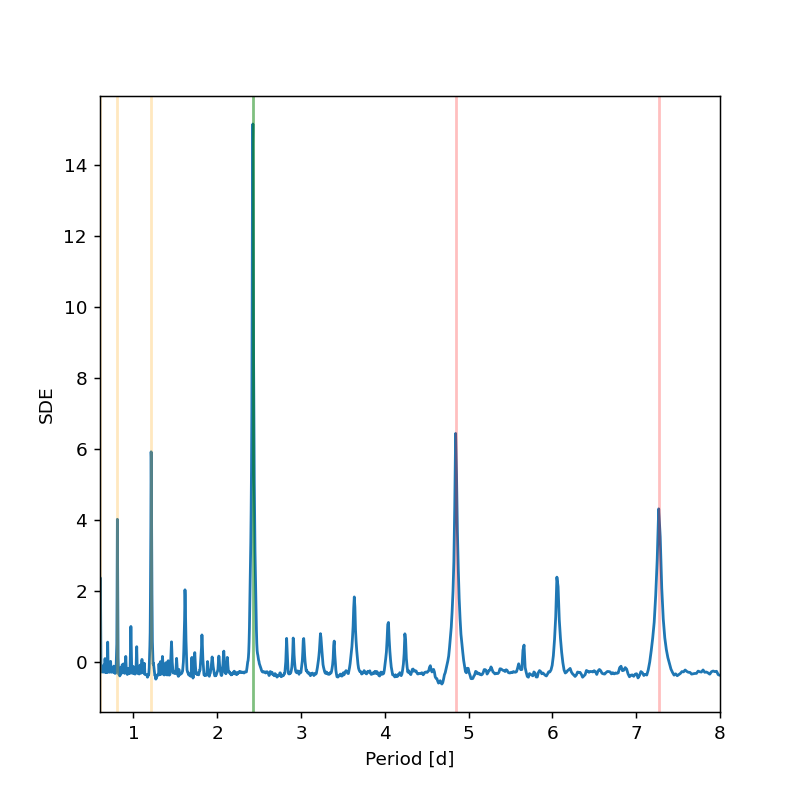
\includegraphics[scale=0.25, angle=0]{pictures/sde.png}
    \caption{TLS periodogram is very clean, ensuring effective transit detection.}
    \label{fig:TLS_periodogram}
\end{figure}
\begin{figure}[h]
  \centering
    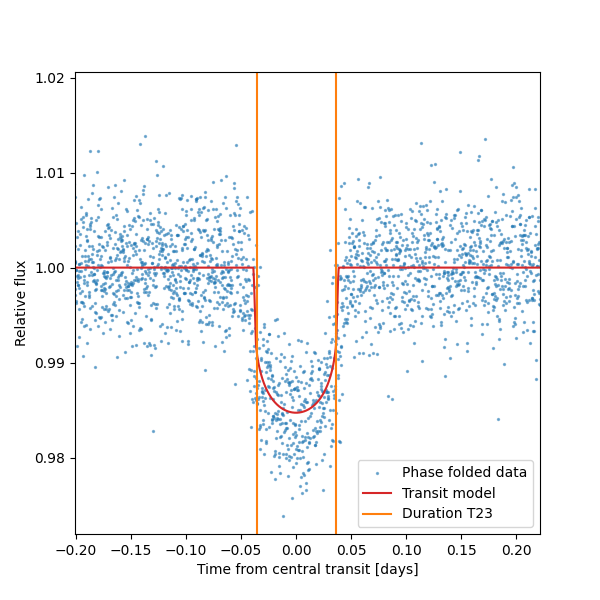
\includegraphics[scale=0.35, angle=0]{pictures/transit_zoom.png}
    \caption{Detrended transits}
    \label{fig:detrended_transits}
\end{figure}
At last, we chose to select only the data points that are at a distance which is within twice the value of the transit duration from the center of the transit. This is just a technicality to save time in the next part of the analysis (PyORBIT run). We saved the output in a data file that will be the basis for the subsequent analysis and we plotted the resulting transit light curve in Fig.\ref{fig:final}.
\begin{figure}[h]
  \centering
    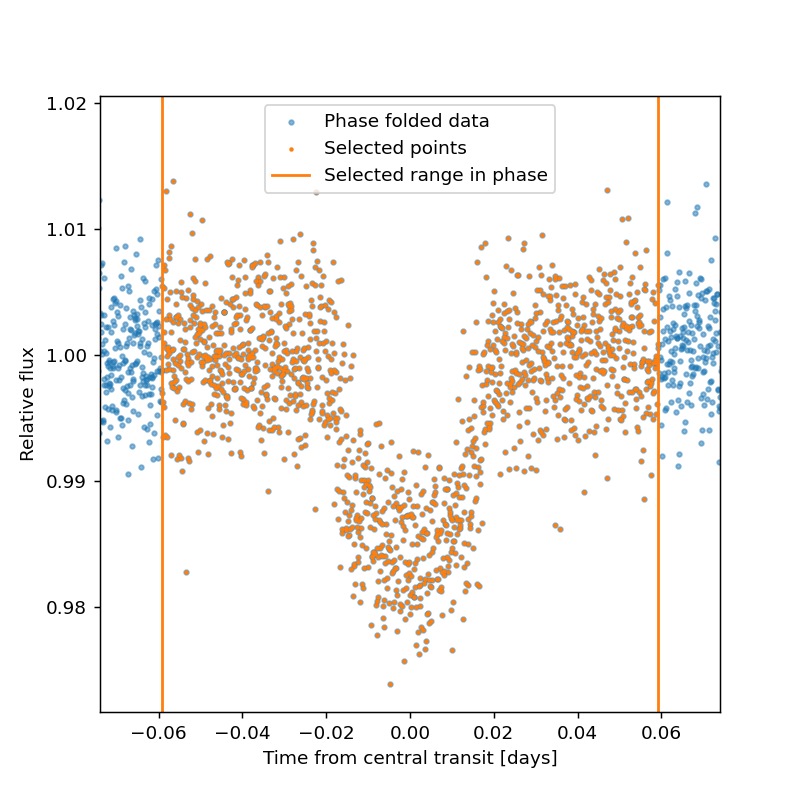
\includegraphics[scale=0.25, angle=0]{pictures/final.png}
    \caption{Final selection}
    \label{fig:final}
 %  \label{fig:Transits}
\end{figure}

\section{Light curve fit}

%Conversion from fit parameters to physical parameters
Once obtained the dataset and prepared the .yaml configuration file for TESS analysis,
%both for TASTE and TESS, 
we fitted the transit light curve with a planetary model. Afterwards we proceeded to repeat the whole procedure for TASTE using the TESS results as priors.
We performed both analysis using \textit{PyORBIT}\footnote{https://github.com/LucaMalavolta/PyORBIT} 
(\cite{Malavolta16}, \cite{Malavolta18}), a framework for the characterization of planetary systems that is able to analyse photometry, 
RVs and ancillary data and to model stellar activity and transit time 
variations.

All the planetary transits were modelled using the Python package 
\textit{BATMAN} (\cite{Kreidberg}); we used also the differential 
evolution tool \textit{PyDE}\footnote{https://github.com/hpparvi/PyDE} 
to perform global optimization of the input parameters in combination with the affine-invariant Markov chain Monte Carlo (MCMC) sampler \textit{EMCEE} (\cite{Foreman}), which took the results of \textit{BATMAN} as starting points for the chains.  Autocorrelation analysis of the chains is also performed. Both for TASTE and TESS, we ran a total of 100000 chain steps, 
from which we cut 20000 steps as burn-in transient phase.
In the configuration files of both analyses the orbits were assumed to be tidally circularized, meaning $e=0$, conventionally associated to a an argument of the pericenter $\omega=\pi/2$. A jitter flag was activated in order to add a jitter parameter in quadrature to the flux errors to compensate for their under-estimation. Finally, we model the limb darkening coefficients with a quadratic law, using Kipping parametrization (\cite{Kipping}).


\subsection{TESS Data Analysis}
For the Bayesian analysis of the TESS lightcurve, we assumed a circular 
orbit, and uniform priors for the period and the central time of transit. $P$ and $T_c$ were given symmetric intervals centered in the TLS estimates, in order to define boundaries for the MCMC analysis: we picked $\delta_P=0.1\cdot P_{TLS}$ and $\delta_{T_c}=1/2\tau$ as semi-intervals. Uniform priors were also assigned to the impact parameter and the scaled planetary radius. Gaussian priors based on the literature were instead settled for the stellar parameters (mass, radisu, density). Limb darkening coefficients are left to vary freely. Since the resulting chains were more than 50 times longer than the 
autocorrelation function, we are assured that the estimate can be trusted.
The physical and derived parameters obtained from the posterior samples are collected in table \ref{table:1}. It should be noticed that the planetary parameters are compatible with literature. In particular TESS period $P=2.42385\pm0.00017$ is compatible with  $P=2.423802^{+0.000032}_{-0.000030} d$ (\cite{Addison}) and $P=2.4238120\pm-0.0000012 d$ (\cite{Turner}) within 1$\sigma$. As for the scaled planetary radius, TESS estimates yields $(R_p/R_{*}) = 0.1170_{-0.0026}^{+0.0025}$, compatible with Harris V filter observation $(R_p/R_{*})=0.1164\pm0.0017$ by \cite{Turner}. Finally, orbital inclination $i$ is compatible with $i=85.98_{0.35}^{+0.39}$ by \cite{Addison}.
%compatible with Addison estimate $(R/R_{*}) = 0.1255\pm 0.0021 $.
% estimates from addison and turner belong to different filters
 \begin{table}[h!]
 \small
 \centering
 %\resizebox{\columnwidth}{!}{%
    \begin{tabular}{cc}
    \hline
    Physical & Value \\
    \hline
    P ($d_{BJD}$)   &  $2.42385\pm0.00017$ \\
    $T_{c} (d_{BJD})$ &  $2458386.57819 _{-0.00070}^{+0.00073}$ \\ 
    $b$ & $0.526_{-0.052}^{+0.047}$ \\
    $R_{P }/ R_{\star}$&  $0.1170_{-0.0026}^{+0.0025}$\\
    $\rho (\rho_{\odot})$ & $1.211_{-0.089}^{+0.088}$\\
    $c1_{ld}$ & $0.51_{-0.28}^{+0.26}$ \\
    $c2_{ld}$ & $0.17_{-0.39}^{+0.40}$\\
    $\sigma_{jit}$ & $0.00024_{-0.00014}^{+0.00022}$ \\
    \hline
    \\
    \hline
    Derived & Value \\
    \hline
    $i (\degree)$ & $86.27^{+0.43}_{-0.42}$ \\
    $R_P/R_J$ &   $1.057\pm0.027$\\
    \hline
    \end{tabular} 
 %}
  \caption{Physical and derived parameters obtained from TESS analysis}
 \label{table:1}
 \end{table}
The corner plots of the posterior samples showing the correlation between 
the parameters are reported in \ref{sect:app_C_TT}.
The normalized stellar fluxes, fitted with the model of the exoplanetary 
transit, along with the residuals are reported in Fig.\ref{fig: lc1}.
\begin{figure}[h!]
    \hspace{-20pt}
    \centering
    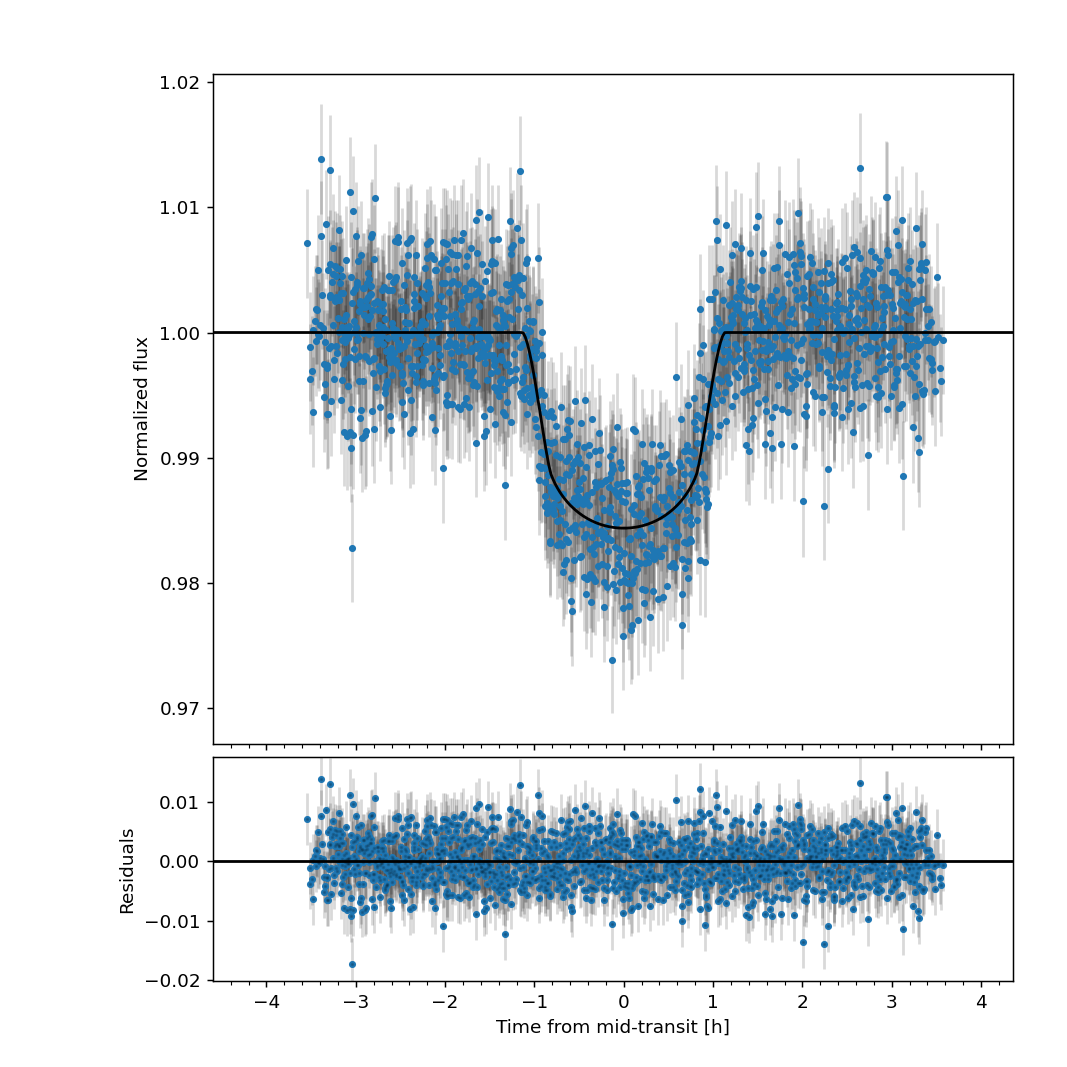
\includegraphics[scale=0.25, angle=0]{pictures/lctess.png}
    \caption{TESS lightcurve}
   \label{fig: lc1}
\end{figure}
Concerning limb darkening coefficients, we can compare these outputs to the models introduced by Claret. \cite{claret2017} and \cite{claret2018} present LD models related to TESS filter. In the above analysis, no prior was used for LD coefficients estimates, making them independent on Claret models. The comparison between such estimates (table \ref{table:1}) and and both \cite{claret2017} and \cite{claret2018} (see \ref{sect:app_A}) shows pretty different results. However, TESS estimates have errorbars large enough to make such results compatible. 


\subsection{TASTE Data Analysis}
As for TASTE lightcurve, we chose a second order 
polynomial trend as a model for out of transit flattening, TESS 
priors for the period, \cite{claret2011} priors for the limb darkening coefficients, gaussian priors for the stellar 
parameters and uniform priors for all the other parameters. Since the resulting chains were more than 50 times longer than the 
autocorrelation function, we are again confident that the estimate can be trusted.

The physical and derived parameters obtained from the posterior 
samples are collected in table \ref{table:2}. As expected, the period is perfectly compatible with the TESS fit value.
%TASTE yields a scaled planetary radius $(R_p/R_{*}) =0.1283 \pm 0.0035$, compatible with \cite{Addison} and \cite{Turner}. (DIFFERENT FILTERS)
%Anderson estimate $(R/R_{*}) = 0.1260\pm 0.0030$.
 \begin{table}[H]
 \small
 \centering
 %\resizebox{\columnwidth}{!}{%
    \begin{tabular}{cc}
    \hline
    Physical& Value \\
    \hline
    P ($d_{BJD}$)   &  $2.42385\pm0.00017$ \\
    $T_{c} (d_{BJD})$ &  $2459174.31781 \pm 0.00057$ \\ 
    b & $0.553_{-0.042}^{+0.038}$ \\
    $R_{P }/ R_{\star}$&  $0.1283 \pm 0.0035$\\
    $\rho (\rho_{\odot})$ & $1.168_{-0.089}^{+0.091}$\\
    $c1_{ld}$ & $0.51\pm0.013$ \\
    $c2_{ld}$ & $0.1699 \pm 0.0060$\\
    $\sigma_{jit}$ & $0.00031_{-0.00036}^{+0.00034}$ \\
    $p_{c0}$ & $1.0538 \pm 0.0010$\\
    $p_{c1}$ &$-0.0019\pm0.0050$\\
    $p_{c2}$ &$-0.58_{-0.22}^{+0.21}$\\ 
    \hline
    \\    
    \hline
    Derived & Value \\
    \hline
    $i (\degree)$ & $86.03_{0.37}^{0.38}$ \\
    $R_P/R_J$ & $1.160^{+0.036}_{-0.035}$\\
    \hline
    \end{tabular} 
 %}
  \caption{Physical and derived parameters obtained from TASTE analysis}
 \label{table:2}
 \end{table}
 %\begin{table}[h!]
 %\small
 %\centering
 %%\resizebox{\columnwidth}{!}{%
 %   \begin{tabular}{cccc}
 %   \hline
 %    Parameter& Value & $\sigma_{-}$ & $\sigma_{+}$\\
 %   \hline
 %   P ($d_{BJD}$)   &  2.455581    &  0.157210  &  0.137465 \\
 %   $T_{c} (d_{BJD})$ &  2459174.317808  & 0.000585   &  0.000574  \\ 
 %   b &  0.557512  & 0.047496    &  0.040594  \\
 %   $R_{P }/ R_{\star}$ & 0.128461 & 0.003655 &  0.003610 \\
 %   $\rho (\rho_{\odot})$ &  1.168443 &0.089728   &   0.091431 \\
%    $c1_{ld}$ &  0.511075    & 0.013099  &  0.013071 \\
 %   $c2_{ld}$ &0.169968 &0.006082 & 0.005921\\
 %   jitter &  0.003081  & -0.000356   & 0.000341\\
 %   $p_{c0}$ & 1.053798  & 0.001009&  0.001041\\
 %   $p_{c1}$ &-0.001874 &0.005019  &0.004961\\
 %   $p_{c2}$ &-0.576007  &0.217093  &  0.212195\\ 
 %   \hline
 %   \end{tabular} 
 %%}
 %  \caption{Physical parameters obtained from TASTE analysis}
 %\label{table:2}
 %\end{table}
Check  \ref{sect:app_C_TT} for corner plots and Fig.\ref{fig: lc2} for the fitted transit.
\begin{figure}[H]
    \centering
    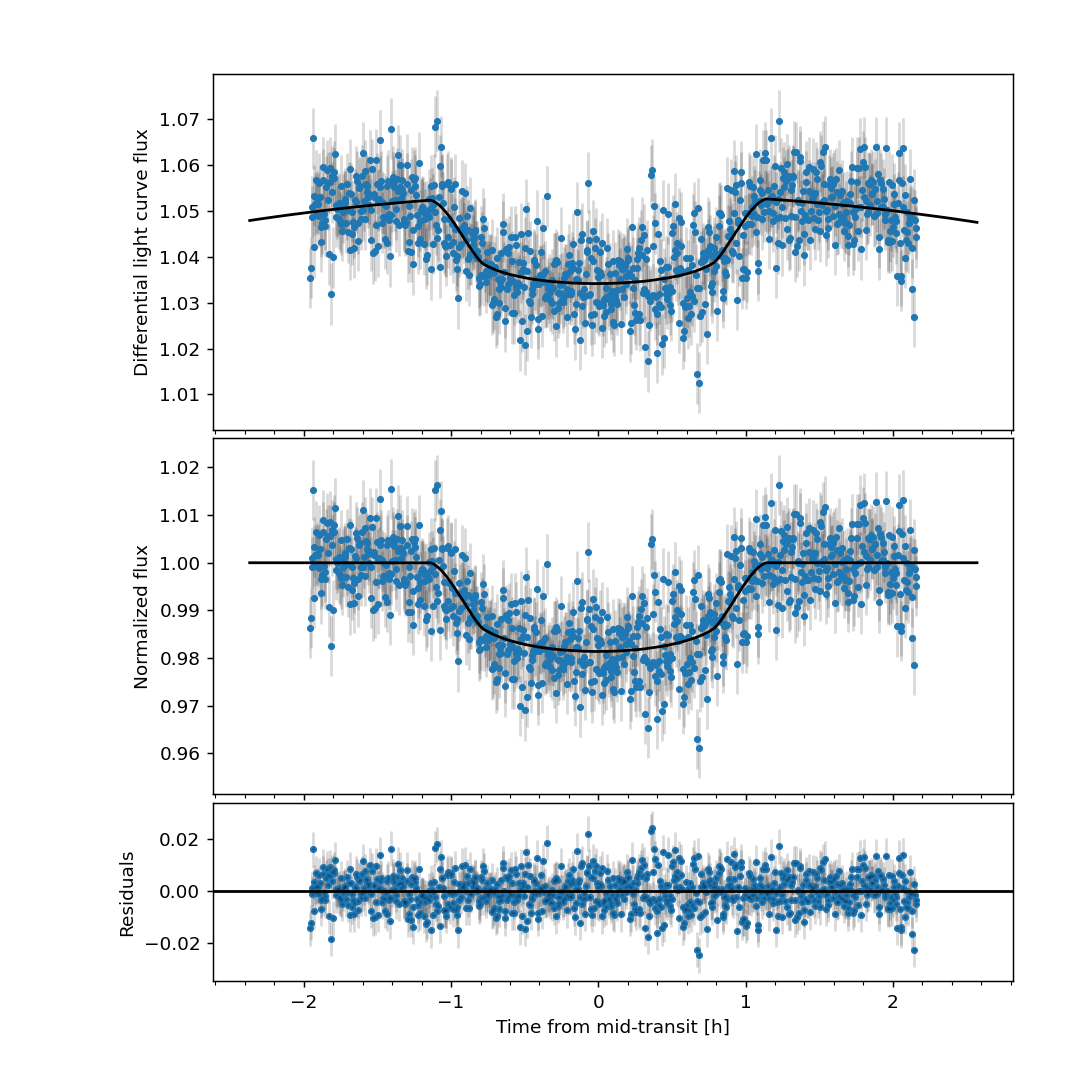
\includegraphics[scale=0.25, angle=0]{pictures/lctaste.png}
    \caption{TASTE lightcurve. Residuals are double those of TESS.}
   \label{fig: lc2}
\end{figure}
 In the configuration file for TASTE, LD quadratic coefficients priors taken from (\cite{claret2011}) were inputted, so TASTE results for $c_1$ and $c_2$ are anchored to that input. Regarding photometry in the same filter ($r'$ from SDSS), \cite{Addison} reports LD coefficients which are largely compatible with Claret 2011 results (see \ref{sect:app_A}).
 




\section{Search for TTV signals}


The transit time variation (TTV) is a sensitive method for the detection of additional planets in compact planetary systems; indeed, in the case of  single-planet systems, the transit in front of the host star is expected at very regular time intervals, hence producing periodic keplerian signals.
Whereas a further unknown planet is present, it will gravitationally perturb the observed transiting planet causing a deviation from its constant periodicity and a departure of the mid transit time from the expected linear keplerian ephemeris.
The amplitude of the TTV signal is proportional to the mass of the perturber and is enhanced in case of low-order (mean motion) orbital resonances between the unknown planet and the transiting one.


%As a further check on the output values of our analysis, 
% we compared the inferred transit times with the linear ephemeris in order to obtain the TTV signal, reported as an observed-calculated diagram
We apply the O-C method in order to compare the observed (O) central transit time (from TASTE observations) to the expected calculated (C) value (TESS results) and to search for any TTV signature.
Linear ephemeris test shows that TASTE has a variation with 
respect to the TESS value $T_c$ propagated in time. The simple calculation 
$$T_c^{calc}=T_c^{TESS}+P\cdot E, \quad E=int\left(\frac{T_c^{TASTE}-T_c^{TESS}}{P}\right)$$
yields $E\approx 525$ (number of cycles) and a variation O-C=$-0.011308 d$ between observed TASTE value and predicted one, that correspond roughly to 16.28 minutes.

\begin{figure}[h]
  \centering
    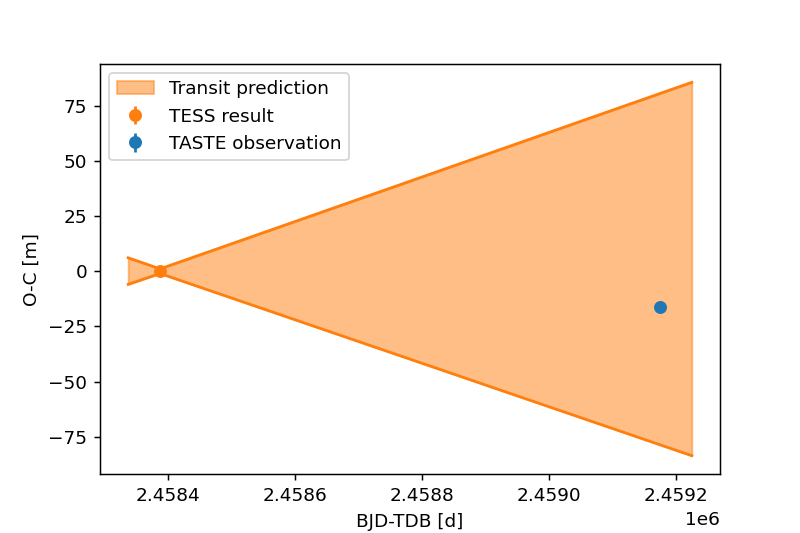
\includegraphics[scale=0.3, angle=0]{pictures/oc.png}
    \caption{O-C plot: checking compatibility between TESS prediction and TASTE result.}
    \label{fig:ocplot}
\end{figure}
The observed-calculated diagram (Fig.\ref{fig:ocplot}) shows the propagation of the error on TESS prediction,
increasing throughout time up to the epoch of TASTE measurement. See 
that TASTE result falls within the cone, proving compatibility of the 
two results. The O-C variation is compatible with the mentioned number of cycles, since errors on $T_c$ propagate through each cycle, so we don't associate such variation to a TTV signal. Therefore from this analysis there seems to be no evidence hinting at the presence of further planets in the planetary system.




\section{Radial velocity analysis}
Knowing the RV semi-amplitude $K_*$ and the mass $M_*$ of the star,
the planetary mass $M_p$ is obtained by inverting the following equation. 
\begin{equation}
    K_* = \frac{1}{\sqrt{1-e^2}}\frac{M_p \sin{i}}{(M_*+M_p)^{2/3}}\left(\frac{P}{2\pi G}\right)^{-1/3}
\end{equation}
where $M_p\sin{i}$ represents a \textit{minimum mass} estimate. $i$ can be 
measured for a transiting planet, thus yielding $M_p$. Between 	July the 1st, 2010 at 08:28 UTC and October the 13th, 2010 at 03:50 UTC the CORALIE spectrograph mounted on the 1.2-m Euler-Swiss telescope in La Silla Observatory was pointed at WASP-44 (\cite{Anderson}). CORALIE is used in conjunction with the Leonhard Euler Telescope to conduct high precision radial velocity measurements, to search for exoplanets in the southern hemisphere. CORALIE is capable of measuring the motion of a star with a precision of about 11km/h (3m/s). It is housed in an isolated and stable environment with regulated temperature to guarantee long-term stability of the measurements. Its design was inspirational for later instruments, as HARPS, which is much more sensible.
For WASP-44, 17 optical spectra were obtained, yielding a RV time series. We made sure the time range of this set did not overlap with the time range of the transits, since that interval is subject to Rossiter-McLaughlin effect.

We ran PyORBIT again to fit the RV curve with a 1-planet model, using N=100000 steps with a burn-in cut of 25000. Inclination was fixed to the value obtained by TESS analysis and Gaussian priors obtained from TESS best-fit values were set on $P$ and $Tc$ .
Radial velocity input data file can be equipped with an extra "0" column (in addition to the one already present accounting for the jitter term), in order to enable the code to compute any RV offset due to the peculiar velocity of the star.
Two models were exploited for the analysis: \textit{radial velocities} and 
\textit{harmonics}. 
%For both models, TESS best-fit values were used as Gaussian priors on period and time of transit.

%The need
We are reasonably impelled to fit two different models since RV signals include planetary signals, 
but also stellar signals. Short-term stellar activity represent a polluting agent, since it is 
induced by spots, rotating with the stellar surface. Given that several active regions rotating 
with the star are present simultaneously on the stellar surface, the observed RV signal 
induced by short-term activity is characterized by signals at the stellar rotation period 
$P$, and its harmonics ($P/2$, $P/3$...). Whenever a signal in the RVs shows a periodicity 
comparable to $P$ or its harmonics, it is very likely induced by active regions. 

%The configuration files for the \textit{PyORBIT} run were prepared with TESS Gaussian priors (already specified)
Results from the two models are collected in tables \ref{table:3} and \ref{table:4}. This observation signals that the mother star $WASP-44$ is pretty inactive, as also shown from CaII observations (\cite{Turner}). 

The simplest model (\textit{radial velocities}) is chosen rather than \textit{harmonics}
because of an unaltered PyORBIT run and slightly smaller errobars. 
The results include an improved result for period $P=2.42381\pm0.00002d$ 
%(compatible with the literature, see \ref{table:0}) 
and a central transit time $T_c=2458386.5782\pm0.0007d$, consistent with TESS prior.
Morevoer, we obtain a radial velocity amplitude $K=137.52^{+10.55}_{-10.09}m/s$
which is fully compatible with the literature value $K=136.5^{+10.0}_{-9.6}m/s$ (\cite{Addison}).
%$K=138.8\pm9.0$ (\cite{Anderson})  
Same for $M_p/M_J = 0.88\pm0.07$, to be compared with  $M_p/M_J=0.860^{+0.072}_{-0.068}$ (\cite{Addison}) and $M_p/M_J=0.867\pm0.064$ (\cite{Turner}).
%$M_p/M_J = 0.89 \pm 0.06$ (\cite{Anderson}),
The huge errorbars found on the jitter term make it far from significative: nothing shows evidence of orbital external perturbation by any gravitational source. The RV offset $v_{off}=-4043.8^{+7.0}_{-6.8}m/s$ is also compatible with $-4045.1^{+7.0}_{-6.2}m/s$ (\cite{Addison}).

We can also derive the planetary bulk  density, BY combining the mass estimate we have just obtained with the radius estimate from TESS (\ref{table:1}): that yields $\rho_p = 0.75\pm0.06$ $\rho_J$. We can take the reference value for Jupiter density \footnote{https://ssd.jpl.nasa.gov/planets}
to be $\rho_J = 1.3262\pm 0.0003 $. Therefore $\rho_p =0.99\pm0.09$ $g/cm^3$, which is compatible with $\rho_p = 0.81^{+0.19}_{-0.16}$ $g/cm^3$ (\cite{Addison}) and $\rho_p = 1.14\pm 0.15$ $g/cm^3$ (\cite{Turner}) within one errorbar. 

The phase-folded RV curves obtained from the fitting with both models 
are reported in \ref{fig:RV1} and \ref{fig:RV2} and the correlation plots 
are collected in \ref{sect:app_C_RV}.  
\begin{table}[H]
    \small
   \centering
    %\resizebox{\columnwidth}{!}{
       \begin{tabular}{cc}
       \hline
        Physical & Value \\
        \hline
		$\sigma_{jit}$ &     $8.38_{-5.76}^{+8.85}$ \\
		$v_{off} (m/s)$ &  $-4043.80_{-6.80}^{+7.00}$ \\
	    $P (d_{BJD})$   & $2.423805\pm0.000021$   \\
	    $T_c (d_{BJD})$  &$2458386.5781\pm0.0007$ \\
	    $K (m/s)$   &$138_{-10}^{+11}$\\
        \hline
        \\
	    \hline 
	    Derived & Value \\
	    \hline
        $M(M_J)$ & $0.88 \pm 0.07$ \\
        $i(deg)$ & $86.28_{0.44}^{+0.43}$\\
       \hline
       \end{tabular} 
%}
     \caption{Physical and derived parameters obtained from \textit{radial velocities} model.}
\label{table:3}
\end{table}
\begin{figure}[H]
	\centering
	%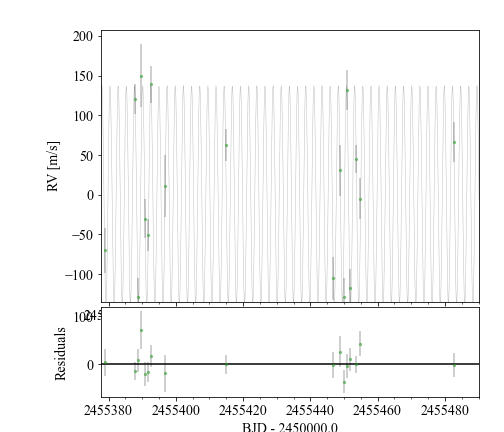
\includegraphics[scale=0.4, angle=0]{../pictures/RV/RV_unfolded.png}
	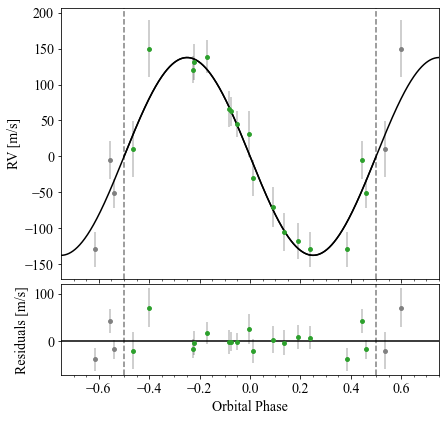
\includegraphics[scale=0.45, angle=0]{pictures/RV.png}
	\caption{Phase-folded curve from the \textit{radial velocities} model. No systematic effect is detected on the residuals, indicating that the model is correctly followed by data, thus proving that the assumption of zero eccentricity and only one planet in the model is compatible with the observations.}
	\label{fig:RV1}
\end{figure}

We also tested the hypothesis that the RV variations
are due to spectral-line distortions caused by a blended eclipsing binary or star spots and changes in the stellar
atmosphere, by performing a line-bisector analysis (\cite{Queloz2001}). Line bisectors are defined as the the loci of the midpoints on the horizontal lines extending from one side to the other of spectral line profiles. The lack of correlation between bisector span (measurement of the inverse of the mean slope of the bisector) and RV (Fig.\ref{fig:bisector}) rules out the null hypothesis and supports another conclusion: the periodic dimming of the flux and the RV variation of the system are due to the reflex
motion of the star caused by the presence of the transiting planet.
\begin{figure}[H]
	\centering
	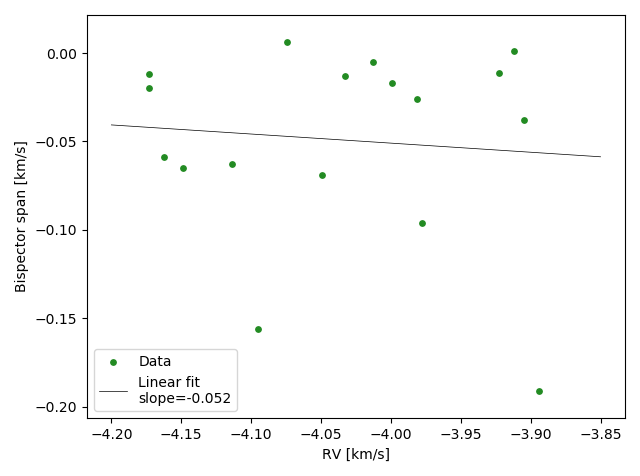
\includegraphics[scale=0.45, angle=0]{pictures/bisector.png}
	\caption{RV data vs line bisector span.}
	\label{fig:bisector}
\end{figure}



In the case of the \textit{harmonics} model, a warning by PyORBIT stated 
that MC chains were too short. This probably means that we did not 
achieve a stationary distribution in the MCMC algorithm, therefore the 
estimates and the autocorrelation function should be treated carefully.
\begin{table}[H]
    \small
	\centering
     %  \resizebox{\columnwidth}{!}{
	\begin{tabular}{cc}
		\hline
		Physical & Value \\
		\hline
		$\sigma_{jit}$ & $ 8.57_{-5.79}^{+9.20} $ \\
		$v_{off} (m/s)$ & $  -4043.89_{-7.05}^{+7.22} $    \\
		$P (d_{BJD})$   & $2.42_{-0.000028}^{+0.000030}$  \\
		$T_c (d_{BJD})$  & $2458386.57820_{-0.00071 }^{+0.00073} $\\
		$K (m/s)$   & $136.20_{-15.24}^{+12.97} $  \\
        \\
        \hline
		Derived & Value \\
		\hline
        $M(M_J)$ & $0.87_{-0.11}^{+0.09}$  \\
        $i (deg)$ & $86.27_{-0.42}^{+0.43} $ \\
		\hline
		%Stellar par& Value & $\sigma_{-}$ & $\sigma_{+}$\\
		%\hline
		%$P (d_{BJD})$ &      2.423846 &        0.000171  &      0.000170\\
		%$phase$ &        6.224110  &        2.214455 &        2.098655  \\
		%\hline
	\end{tabular} 
%}
	\caption{Physical and derived parameters obtained from \textit{harmonics} model.}
\label{table:4}
\end{table}
\begin{figure}[H]
	\centering
%	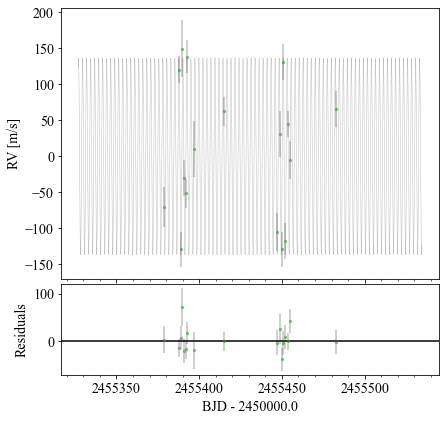
\includegraphics[scale=0.4, angle=0]{../pictures/RV/RV2_unfolded.png}
	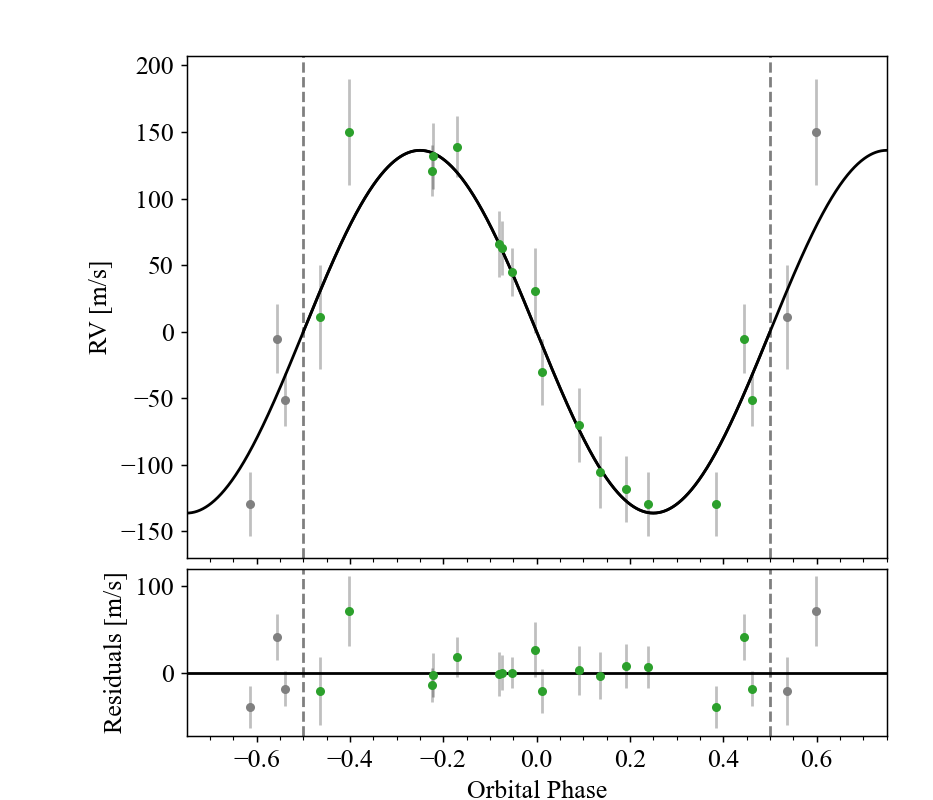
\includegraphics[scale=0.25, angle=0]{pictures/RV2.png}
	\caption{Phase-folded radial velocity curve from the \textit{harmonics} model.}
	\label{fig:RV2}
\end{figure}

%\section{Temp}

%\begin{figure}[H]
%  \centering
%  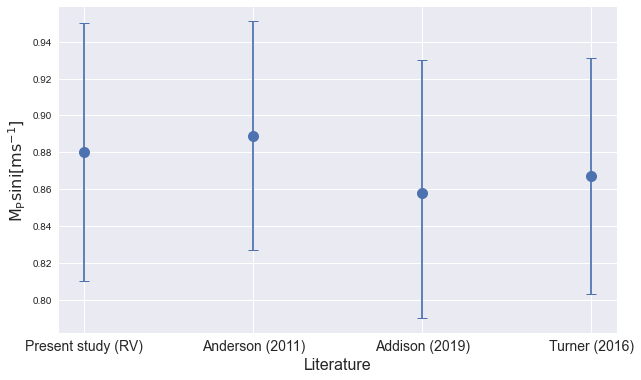
\includegraphics[width=.8\linewidth]{pictures/mass.png}  
%  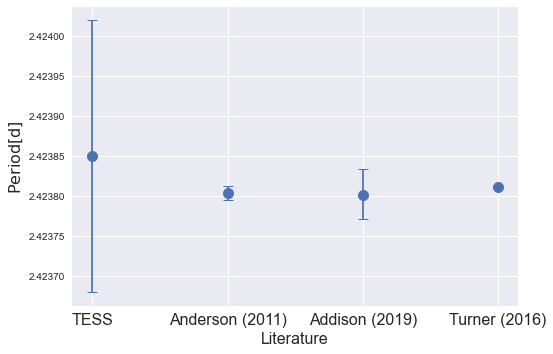
\includegraphics[width=.8\linewidth]{pictures/period.png} 
%  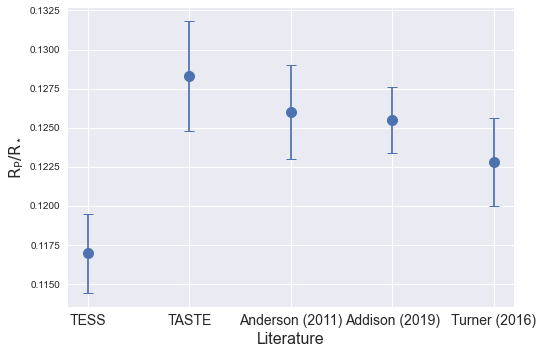
\includegraphics[width=.8\linewidth]{pictures/radius.png}  
%  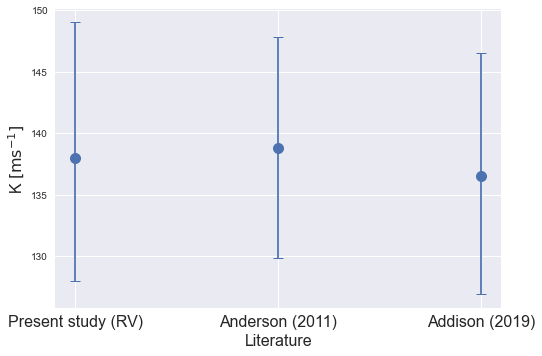
\includegraphics[width=.8\linewidth]{pictures/K.png}  
%\caption{Comparison with the literature}
%\label{fig:temp}
%\end{figure}


\section{Conclusions}

%we compared the inferred transit times with the linear ephemeris in order to obtain the TTV signal, reported as an observed-calculated diagram

The main goals of this work were to extract the lightcurve both from ground-based TASTE observations and TESS space data, to compute mid-transit time of TESS (reliable because obtained from several transits) and TASTE and to check whether the latter falls inside the propagated prediction of the former, with the aim of searching for a TTV signal between the prediction of the linear ephemeris and the observations in the reported O-C diagram.  
No significant evidence for a possible transit time variation was detected.
%This is verified by \ref{fig:ocplot} so the estimates are compatible.

A comparison with the literature is also due: compatibility was found for the period and for the scaled planetary radius estimated from TESS data.
%retrieved from TASTE observations. 

In addition to the photometric analysis, RV data from CORALIE were exploited to enable a mass estimate. Reasonable agreement with the literature were obtained for the planetary mass, the bulk density and the radial velocity amplitude; furthermore the phase-folded RV curve residuals showed no significant systematic trends. 
%0.881943 0.105127 0.074306

WASP-44 b is a planet with mass $M_P=0.88\pm0.07 M_J$, 
%scaled radius $(R_p/R_{*})=0.1170_{-0.0026}^{+0.0025}$,
radius $R_p=1.057\pm0.027 R_{J}$,
bulk density $\rho_p =0.99\pm0.09$ $g/cm^3$ and orbits with a period of $P=2.423805\pm0.000021d$ around a pretty inactive parent star. 
%For the period, I put the improved value from RV analysis, based on TESS prior
In conclusion, no evidence of orbital perturbation due to an extra planetary body was 
found.


\printbibliography
\nocite{*}

\onecolumn

\appendix
\section{Limb darkening analysis}
\label{sect:app_A}

\subsection{Claret 2017}
We can represent data tables in \cite{claret2017} as 2D histograms, 
after proper unfolding of the data tables attached to the paper. To do that, 
we first fix metallicity, then gravity and see how the corresponding LD 
coefficients $c_1$ and $c_2$ depend on all three atmospheric parameters. 
\begin{figure}[h]
    \centering  
    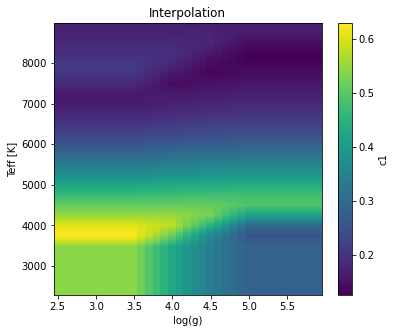
\includegraphics[scale=0.4, angle=0]{pictures/2017_c1_fixedmet}
    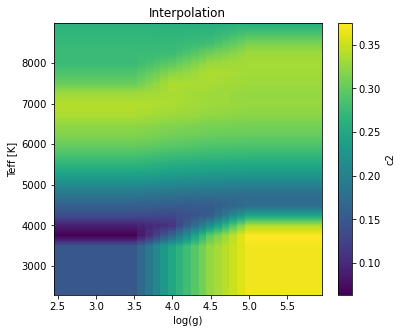
\includegraphics[scale=0.4, angle=0]{pictures/2017_c2_fixedmet}

    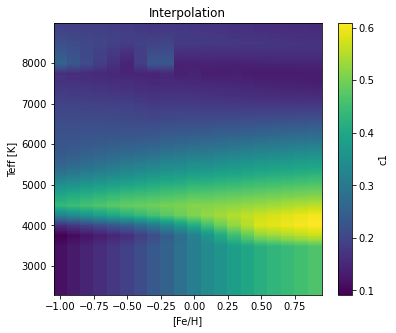
\includegraphics[scale=0.4, angle=0]{pictures/2017_c1_fixedg}
    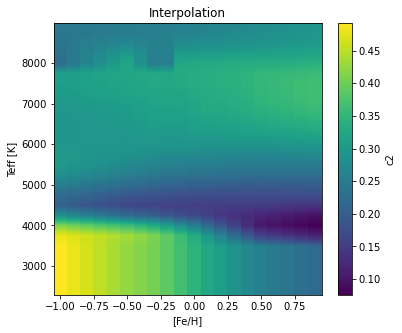
\includegraphics[scale=0.4, angle=0]{pictures/2017_c2_fixedg}
    \caption{LD coefficient with fixed metallicty (top panels), fixed gravity (bottom panels)}
\end{figure}
We immediately visualize a vertical gradient rather than a horizontal one,
showing that temperature dependence is very strong. Turns out LD 
coefficients are essentially a function of temperature, and minor 
dependences on gravity and metallicity can be barely appreciated.
\begin{figure}[h]
    \centering  
    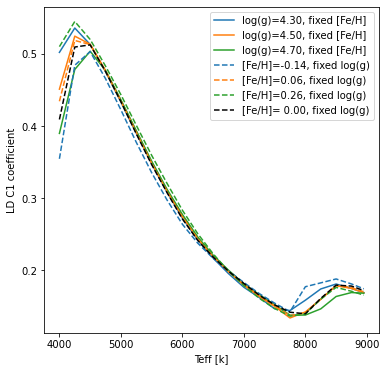
\includegraphics[scale=0.4, angle=0]{pictures/2017_c1}
    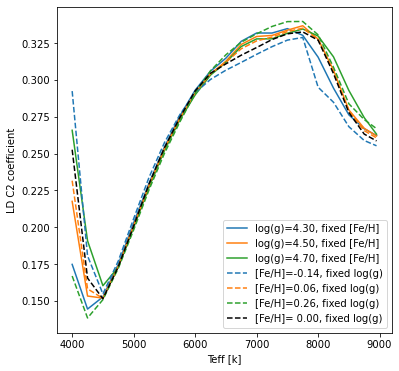
\includegraphics[scale=0.4, angle=0]{pictures/2017_c2}
    \caption{LD coefficient as a function of atmospheric parameters. Curves deviate at $T\leq 4500K$ and $T\geq 8000K$. Central part of the function is not sensitive to gravity and metallicty, both for $c_1$ and $c_2$.}
\end{figure}
A relevant dependance on gravity and metallicity can only be noticed at 
high temperatures, where we should carefully select the proper curve. However,
in the range we're interested in ($\approx 5400 K$) the curve is 
degenerate and the choice of these parameters is secondary.

We perform a Montecarlo simulation, generating 1000 random atmospheric 
parameters around the actual ones, using the reference errorbar, 
thus conserving the error scale. This expedient will enable us 
to consider the result of this analysis as a good physical 
estimate of the LD coefficients. 
Even in this case we see that the 
distribution of the fixed-metallicity estimates is almost overlapping 
with the fixed-gravity one, thus confirming that, according to the 
exploited table, $c_1$ and $c_2$ not very sensitive on metallicity and gravity.
\begin{figure}[h]
    \centering  
    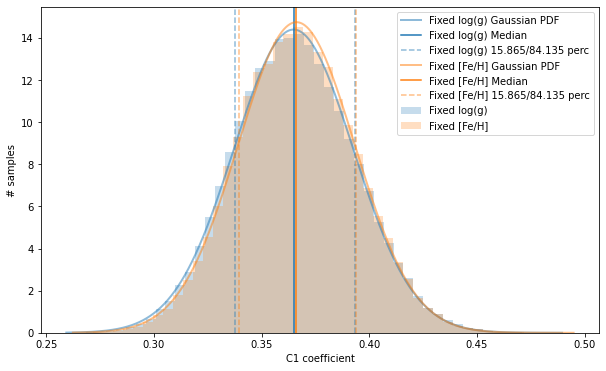
\includegraphics[scale=0.35, angle=0]{pictures/2017_c1_comp}
    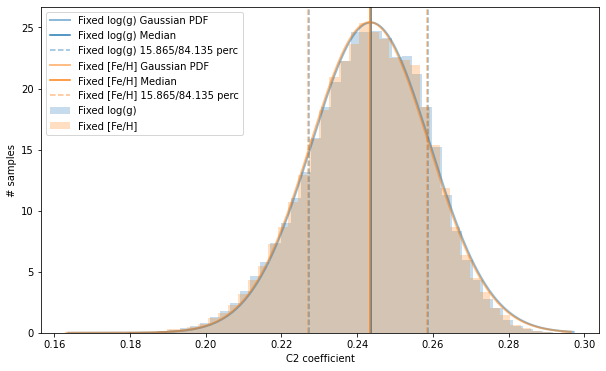
\includegraphics[scale=0.35, angle=0]{pictures/2017_c2_comp}
    \caption{Montecarlo simulation for $c_1$ (left) and $c_2$ (right), 
    for fixed metallicity and for fixed gravity.}
\end{figure}
\begin{table}[h!]
	\centering
	\begin{tabular}{ccccc}
		\hline
		& $c_1$ & $\sigma_{c1}$ & $c_2$ & $\sigma_{c2}$\\
		\hline
		Fixed $[Fe/H]$ Median   & 0.3662 & 0.0271 & 0.2433 & 0.0157\\
		Fixed $\log{g}$ Median: & 0.3648 & 0.0277 & 0.2436 & 0.0157 \\
		\hline
	\end{tabular} 
\end{table}
For both coefficients, the two estimates coming from metallicty and 
gravity fixing are well compatible, thus authorizing a weighted average: 
$c_1 = 0.366 \pm 0.019$ and $c_2 = 0.243 \pm 0.011$.

\medskip

Another way to deal with the same table is by selecting from the set two values
of metallicity or gravity, an upper and lower limit, instead of just one reference 
value. This way we build two matrices and 
interpolate between the two to get to the desired result. The rest of the 
procedure is identical, leading to similar estimates of the LD coefficients.
\begin{figure}[h!]
    \centering  
    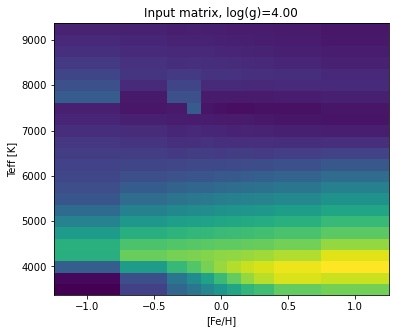
\includegraphics[scale=0.35, angle=0]{pictures/double_logg4}
    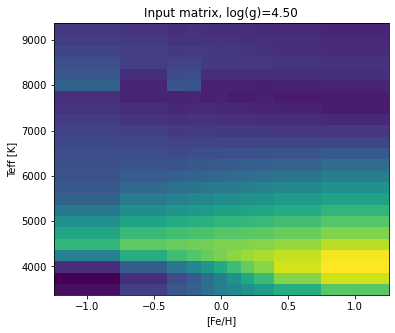
\includegraphics[scale=0.35, angle=0]{pictures/double_logg45}
    \includegraphics[scale=0.35, angle=0]{pictures/double_logg_interp}
    \caption{Matrices obtained by fixing gravity to $\log{g}=4.0$ and to $4.5$, plus the interpolated matrix}
\end{figure}
\begin{figure}[h!]
    \centering  
    \includegraphics[scale=0.4, angle=0]{pictures/double_c1}
    \includegraphics[scale=0.4, angle=0]{pictures/double_c2}
    \caption{LD coefficients trend in the $T_{eff}-[Fe/H]$ plane}
\end{figure}
Degeneracy is less pronounced if we treat data this way. In fact, changing 
secondary atmospheric parameters ($g$ and $[Fe/H]$) now produces a still 
modest, but visible scatter. This is confirmed by the Montecarlo analysis, 
that yields results compatible with the previous case but with larger errorbars.
\begin{table}[h!]
	\centering
	\begin{tabular}{ccccc}
		\hline
		& $c_1$ & $\sigma_{c1}$ & $c_2$ & $\sigma_{c2}$\\
		\hline
		Fixed $\log{g}$ Median: & 0.3650 & 0.0276 & 0.2436 & 0.0156 \\
		\hline
	\end{tabular} 
\end{table}
The procedure could be repeated in the same way by fixing metallicity instead.




\subsection{Claret 2018}
A followup paper (\cite{claret2018}) provided a new method to model the LD coefficients dependency 
on atmospheric parameters. We'd like to check if this leads to different results 
with respect to \cite{claret2017}. Unfolding the table requires the same procedure 
we've already described. Just note that in both cases we fix metallicity, and for 
the 2018 table metallicity must be fixed to 0, since the method is conceived for
zero-metallicity stars.
\begin{figure}[H]
    \centering  
    \includegraphics[scale=0.4, angle=0]{pictures/2017.png}
    \includegraphics[scale=0.4, angle=0]{pictures/2018.png}
    \caption{Comparison between interpolated matrices at fixed metallicity, to the 
    stellar metallicity (2017 left), and to 0 (2018 right).}
\end{figure}
And finally we can display the dependency of the LD coefficients for the 
two-parameters game.
\begin{figure}[H]
    \centering  
    \includegraphics[scale=0.4, angle=0]{pictures/c1.png}
    \includegraphics[scale=0.4, angle=0]{pictures/c2.png}
    \includegraphics[scale=0.35, angle=0]{pictures/c1_comp.png}
    \includegraphics[scale=0.35, angle=0]{pictures/c2_comp.png}
    \caption{$c_1$ and $c_2$ trend, and comparison between the final results. Gaussian bells of the 2018 model are narrower.}
\end{figure}
First, the degeneracy on $g$ and $[Fe/H]$ is completely removed, so that they 
can no longer be referred to as "secondary parameters". The comparison above shows 
that choosing the model will influence, even strongly, the estimate of 
the parameters. Quantitatively, the region characterised by $T\approx5400 K$
is one of the least affected by model choice, but the difference is still 
too wide to be neglected.
The final estimates for the parameters are also quite different, both in 
terms of value and in terms of error. This indicates a systematic difference 
caused by the choice of the model. Because of this, we need to artificially 
inflate the error before using limb darkening parameters. This is very 
important especially for shallow transits like ours.
Anyway, they're largely compatible still: see how each value is within a 
few errorbars away from the other.
\begin{table}[h!]
	\centering
	\begin{tabular}{ccccc}
		\hline
		& $c_1$ & $\sigma_{c1}$ & $c_2$ & $\sigma_{c2}$\\
		\hline
		2017 Median & 0.3631 & 0.0272 & 0.2444 & 0.0157 \\
		2018 Median & 0.3961 & 0.0155 & 0.2030 & 0.0048 \\
		\hline
	\end{tabular} 
\end{table}
The model from \cite{claret2018} yields results with 
smaller errorbars for both coefficients.



\subsection{Claret 2011}
We use another table from an older paper (\cite{claret2011}) by the same author, 
this time including filters. The header of our dataset shows that the filter $r^{*}$
was used (SDSS). Remember that transits look differently 
when observed through different filters, and also that boxier transits make 
ingress/egress time determination easier. $r^*$ filter was selected
(SDSS), since it
is the best choice in terms of CCD efficiency and
in terms boxiness of the transit, making it eas-
ier to determine ingress and egress time, and
therefore central time of transit.
The unfolding technique of the 
data pack is always the same.
This time, we account for stellar models (ATLAS/PHOENIX) and interpolation 
technique (least squares/flux conservation), for a grand total of 4 
combinations. These are the very final results.
\begin{figure}[H]
    \centering  
    \includegraphics[scale=0.4, angle=0]{pictures/c1.png}
    \includegraphics[scale=0.4, angle=0]{pictures/c2.png}
    \includegraphics[scale=0.35, angle=0]{pictures/c1_comp.png}
    \includegraphics[scale=0.35, angle=0]{pictures/c2_comp.png}
    \caption{$c_1$ and $c_2$ trend, and comparison between the final results}
\end{figure}
Again, see how the choice of the model is deeply influencing the trend of 
the coefficients with respect to the atmospheric parameters, and the results 
consequently. 
\begin{table}[h!]
	\centering
	\begin{tabular}{ccccc}
		\hline
		& $c_1$ & $\sigma_{c1}$ & $c_2$ & $\sigma_{c2}$\\
		\hline
		ATLAS, LS:      & 0.4701 & 0.0367 &0.2327 &0.0231 \\
		ATLAS, FC:      & 0.4848 & 0.0347 & 0.2142 &  0.0205 \\
		PHOENIX, LS:    & 0.5251 & 0.0219 & 0.1728 & 0.0098 \\
		PHOENIX, FC:    & 0.5434 & 0.0212 &  0.1499 & 0.0088 \\
        \hline
	\end{tabular} 
\end{table}
Despite being compatible between each other, the estimates of 
the coefficients are quite detached from the one inferred following 
\cite{claret2017} and \cite{claret2018}. This reinforces the need to add 
a systematic error term. 


Note that changing stellar model means changing the
way we compute the gradient of temperature
and the flux in stellar photosphere. 
In our case, Phoenix stellar model seems to be associated with 
slightly thinner errorbars, but the difference form ATLAS is not 
a relevant one.




\newpage
\section{Time correction}
\label{sect:app_B}

When reducing TASTE data and dealing with \textit{sentinel.dat} output, we need to properly convert the 
time series, contained in columns two of the datatable. To do that, first we
convert from minutes to days, then add the zero-point in Julian Date format, and 
finally also add half exposure time (after proper conversion in days).

Moreover, we can make use of the \textit{Time} method to keep count of the time 
taken by the light to travel from the source position to the location of the 
observatory (Cima Ekar, Asiago). Since the Earth is in motion, light time 
travel is variable and follows a sinusoidal behaviour.
\begin{figure}[H]
    \centering  
    \includegraphics[scale=0.4, angle=0]{pictures/time_corr.png}
\end{figure}

As a result, all times were converted from Julian Days expressed in the Universal Coordinated Time (JD$\_$UTC), which is a geocentric reference frame, into Julian Days in the barycentric reference frame of the Solar System (BJD$\_$TDB), which is given by the sum of the time at the Earth barycenter and the ligh travel time.


\section{Figures}




\subsection{TESS and TASTE}
\label{sect:app_C_TT}

Corner plots are generated as a result of PyORBIT and are plotted using the \textit{corner} package. Along the diagonal there are histograms of the estimated 1D posterior 
probability distribution for each parameter. 
The histograms show that the recovered parameters are both accurate 
(close to injected value) and precise (narrow posterior distribution). 
The off-diagonal plots are the 2D histograms of the estimated joint 
posterior probability distribution of each pair of parameters, which show the correlation between pairs of parameters. The gray-scale map indicate the density of samples derived from MCMC simulation.

\begin{figure}[H]
    \centering
      \includegraphics[scale=0.18, angle=0]{pictures/corner_tess.png}
       \caption{Correlation between TESS parameters. Each LD coefficient distribution is a little clumpsy, and also there's evidence for severe correlation between the two. This suggests TESS estimation of LD coefficients is not fully trustworthy.  More data could make corner plots more significant. Little anti-correlation is found between period and central time of transit, as weel as little correlation between impact parameter and scaled radius. }
%      \label{fig: cptess}
\end{figure}

\begin{figure}[H]
    \centering
      \includegraphics[scale=0.18, angle=0]{pictures/corner_taste.png}
      \caption{Correlation between TASTE parameters.}
%     \label{fig: cptaste}
\end{figure}

\begin{figure}[H]
  \centering
    \includegraphics[scale=0.4, angle=0]{pictures/poly.pdf}
    \caption{TASTE polynomial trend corner plot}
 %  \label{fig: ptrend}
\end{figure}


%\newpage

\subsection{Radial velocities}
\label{sect:app_C_RV}




\begin{figure}[h]
    \centering
      \includegraphics[scale=0.25, angle=0]{pictures/corner_RV.png}
      \caption{Correlation between parameters of the \textit{radial velocities} model. Evidence of correlation is found for the mass versus velocity amplitude plot. The linear relation between the two implies some degree of degeneracy.}
     \label{fig: cpRV}
\end{figure}

\begin{figure}[h]
    \centering
      \includegraphics[scale=0.25, angle=0]{pictures/corner_RV_harmonics.png}
      \caption{Correlation between parameters of the \textit{harmonics} model}
     \label{fig: cpRV2}
\end{figure}


\end{document}